\chapter{Analyse des Brettspiels}
\label{chapter:analyse-des-bretspiels}

Im folgenden Abschnitt werden zuerst die Spielregeln von Patchwork genauer erläutert. Darauf aufbauend wird das Spiel nachfolgend mit verschiedenen Ansätzen aus der Spieltheorie analysiert, was später für die Erstellung der unterschiedlichen Computergegner relevant ist.

\section{Spielregeln}
\label{section:spielregeln}

Bevor der eigentliche Spielverlauf starten kann, muss das Spiel vorbereitet werden. Hierzu erhalten beide Spieler eine der beiden Decken, auch als Ablageplan bezeichnet, den dazugehörigen Zeitstein und jeweils 5 Knöpfe, welche die Währung im Spiel repräsentieren. Anschließend wird der zentrale Zeitplan in die Mitte des Spielfelds gelegt. Der Zeitplan ist beidseitig mit unterschiedlichen Designs bedruckt, da diese jedoch in allen spielrelevanten Belangen gleich sind, ist die gewählte Seite für den Spielverlauf irrelevant. Die kleinen, braunen Spezialflicken werden jetzt auf den dafür vorgesehenen gedruckten Feldern auf den Zeitplan platziert, welche sich zwischen den Spielfeldern befinden. Nun werden die beiden Zeitsteine der Spieler auf das Startfeld des Zeitplans gestellt. Beginnen darf im Spiel nach dem vollständigen Aufbau des Spielfelds, wer zuletzt eine Nähnadel in der Hand hatte. Daraus ergibt sich, dass bei einem Spiel gegen einen in dieser Arbeit beschriebenen Computergegner, der menschliche Spieler immer mit dem Spiel beginnen muss, da dieser Computergegner noch keine Nähnadeln halten können. Alle Flicken werden nun in einem Kreis oder einer Ellipse um den Zeitplan herum zufällig verteilt und die Spielfigur zwischen dem kleinsten Flicken, der nur zwei Felder auf einem Ablageplan einnimmt, und dem im Uhrzeigersinn folgenden Flicken gesetzt. In der Abbildung \ref{fig:spielaufbau} ist der initialen Spielaufbau des Zeitplans mit reduzierter Flickenanzahl für bessere Übersichtlichkeit zu sehen. Die übrig gebliebenen Knöpfe werden zusammen mit dem Sonderplättchen $7\times7$ als Vorrat bereitgelegt. \cite{2014.PatchworkSpielanleitung}

\pagebreak

\begin{figure}[!ht]
    \centering
    \begin{tikzpicture}
        \node [inner sep=0pt,,outer sep=0pt,clip,rounded corners=0.15cm] (image) at (0,0) {\includegraphics[width=0.8\textwidth]{res/pictures/game-structure.jpg}};
        \drawshadow{image}
    \end{tikzpicture}
    \caption{Spielaufbau mit reduzierter Flickenanzahl}
    \label{fig:spielaufbau}
\end{figure}

Jetzt kann das Spiel beginnen. Gegensätzlich zu klassischen Spielen sind bei Patchwork die beiden Spieler nicht unbedingt immer abwechselnd an der Reihe. Es ist immer derjenige Spieler an der Reihe, dessen Zeitstein hinter oder auf dem Zeitstein des anderen Spielers steht. Das heißt, wenn der Zug eines Spielers auf dem Feld endet, auf welchem der Zeitstein des anderen Spielers steht, ist der Spieler, welcher soeben gezogen hat, noch einmal an der Reihe. \cite{2014.PatchworkSpielanleitung}

Wenn ein Spieler an der Reihe ist, hat er die Auswahl zwischen zwei verschiedenen Aktionen:

\begin{itemize}
    \item \textbf{Vorrücken und Knöpfe erhalten} \cite{2014.PatchworkSpielanleitung}
    \item \textbf{Flicken nehmen und einfügen} \cite{2014.PatchworkSpielanleitung}
\end{itemize}

Bei der Aktion \textbf{Vorrücken und Knöpfe erhalten} setzt der Spieler seinen Zeitstein so viele Felder vor, bis er sich auf dem Feld vor dem Zeitstein des anderen Spielers befindet. Für jedes Feld erhält der Spieler einen Knopf vom Vorrat. \cite{2014.PatchworkSpielanleitung}

Die Aktion \textbf{Flicken nehmen und einfügen} besteht aus fünf Schritten, welche in der folgenden Reihenfolge durchgeführt werden müssen:

\begin{enumerate}
    \item \textbf{Flicken auswählen}: Der Spieler hat die Auswahl zwischen den nächsten drei Flicken im Uhrzeigersinn nach der Spielfigur. \cite{2014.PatchworkSpielanleitung}
    \item \textbf{Spielfigur setzen}: Der Spieler setzt die Spielfigur neben den ausgewählten Flicken. \cite{2014.PatchworkSpielanleitung}
    \item \textbf{Flicken bezahlen und nehmen}: Der Spieler bezahlt die auf dem Etikett des Flickens angegebene Knopfzahl (in Abbildung \ref{fig:patch-explanation} zu sehen) an den Vorrat und legt den Flicken zu seinem Ablageplan. \cite{2014.PatchworkSpielanleitung}
    \item \textbf{Flicken platzieren}: Der Spieler platziert den Flicken auf seinen Ablageplan mit beliebiger Rotation und Spiegelung. Jedoch dürfen nur freie Felder belegt werden und der Flicken muss vollständig auf dem Ablageplan liegen, sie dürfen also nicht über den Rand des Plans hinausragen. \cite{2014.PatchworkSpielanleitung}
    \item \textbf{Zeitstein ziehen}: Der Spieler zieht seinen Zeitstein so viele Felder nach vorne, wie auf dem Etikett des eben abgelegten Flickens abgebildet sind (in Abbildung \ref{fig:patch-explanation} zu sehen). Ist das letzte Feld des Zuges jenes Feld, auf welchem schon der andere Spieler steht, wird der Zeitstein auf den des anderen Spielers gestellt. \cite{2014.PatchworkSpielanleitung}
\end{enumerate}

\begin{figure}[!ht]
    \centering
    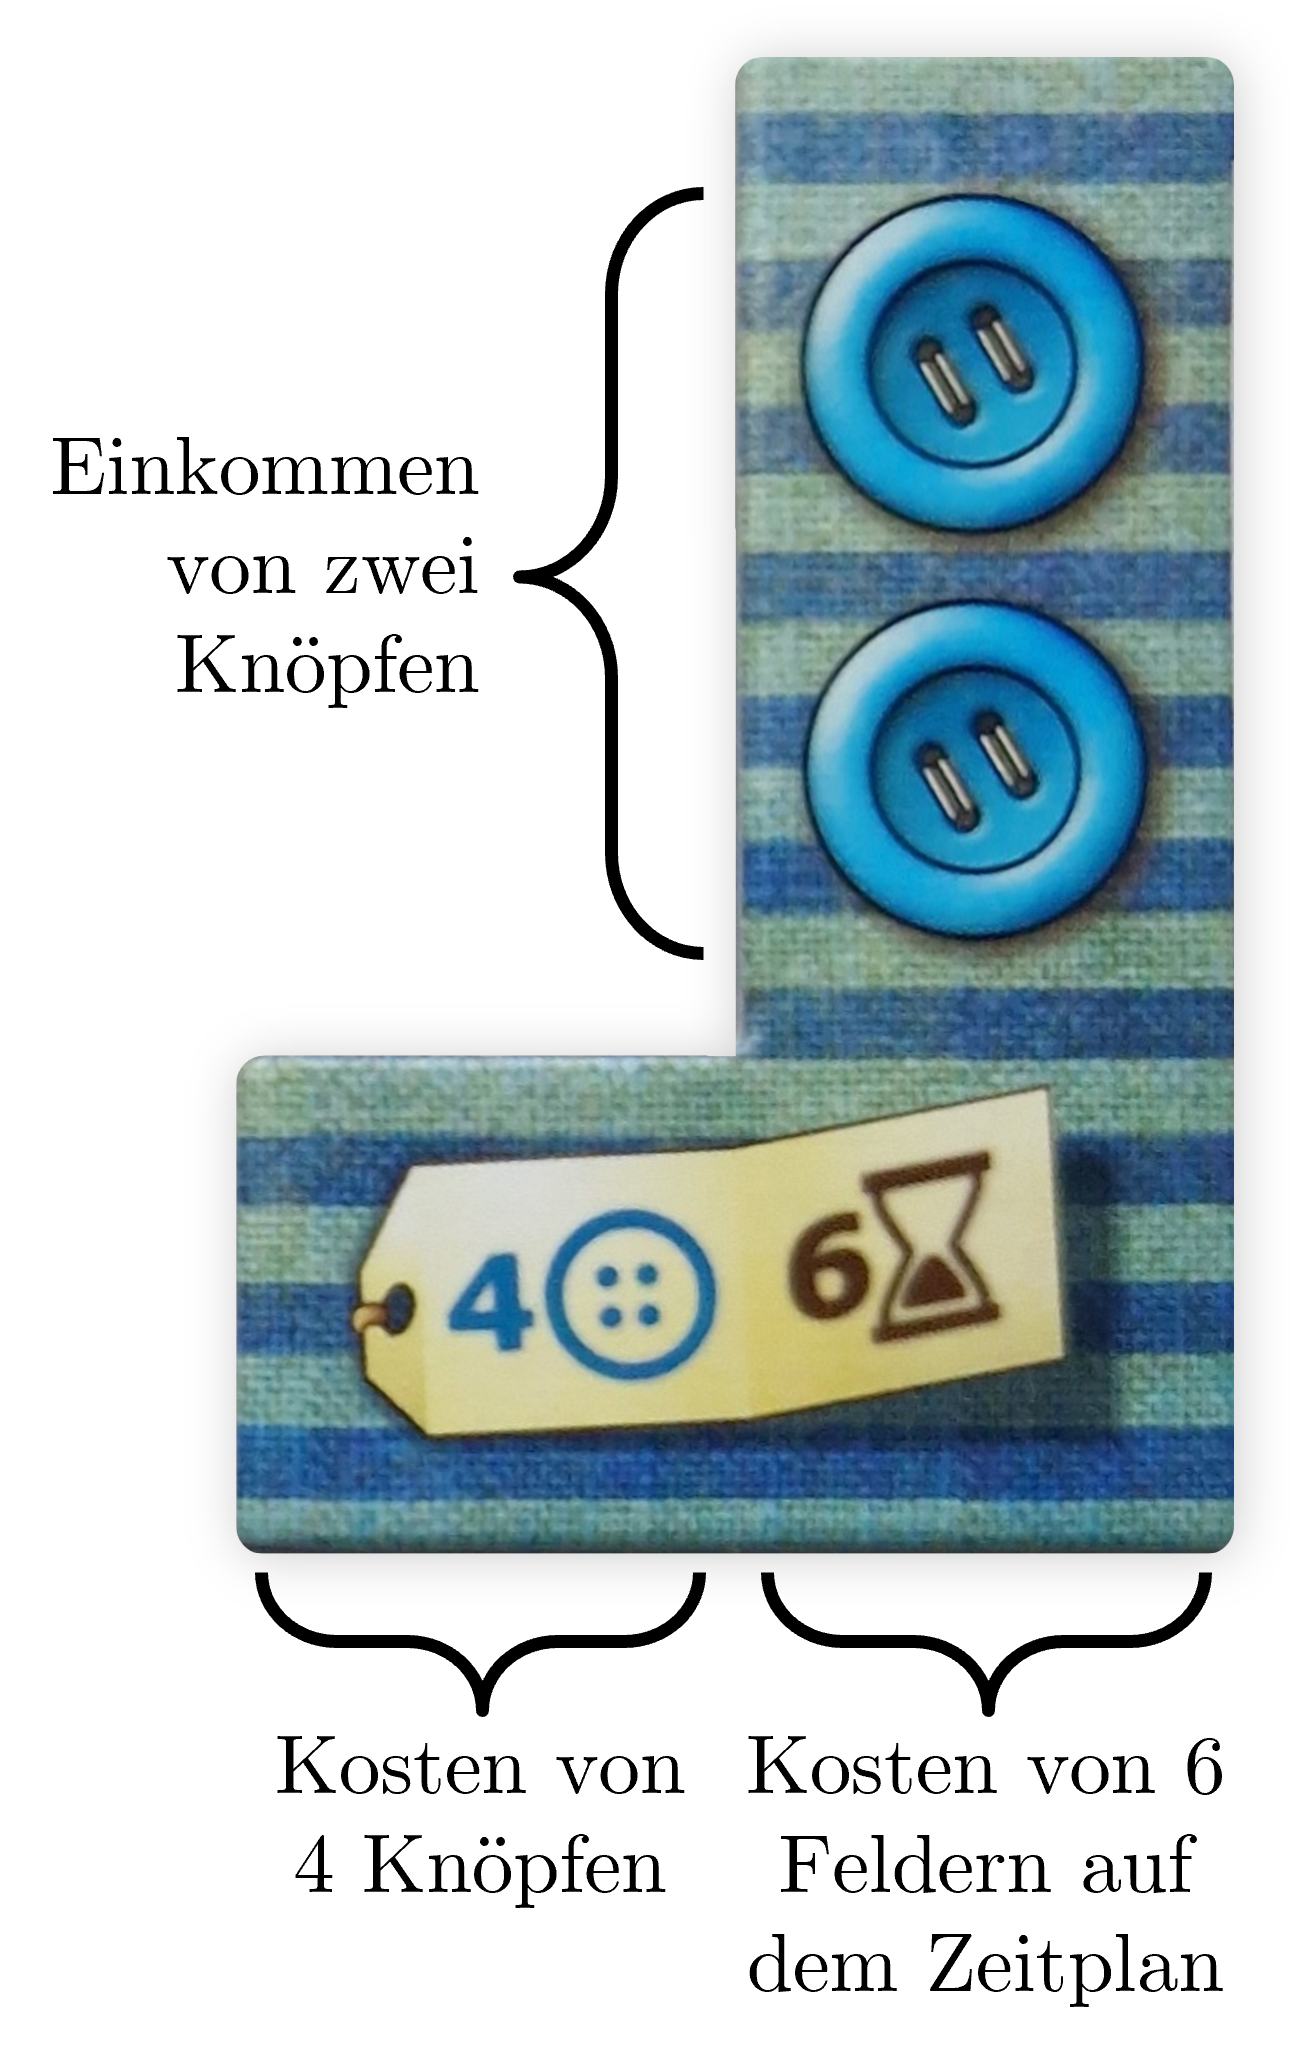
\includegraphics[width=0.3\textwidth]{res/pictures/annotated-patch.png}
    \caption{Flicken mit erklärender Beschriftung}
    \label{fig:patch-explanation}
\end{figure}

Während des Spielverlaufs rücken die Zeitstein der beiden Spieler immer weiter auf der Zeitleiste auf dem Zeitplan vor. Dort sind zwei Markierungen denen Beachtung geschenkt werden muss. Zum einen sind dort die Spezialflicken zu finden, welche der Spieler, der zuerst seinen Zeitstein über einen Spezialflicken zieht, für seinen Ablageplan verwenden und dort ablegen muss. Zum anderen sind Knöpfe auf der Zeitleiste zu erkennen. Wenn ein Zeitstein über ein solchen Knopf gezogen wird, bekommt derjenige Spieler ein Knopfeinkommen vom Vorrat in Höhe der Summe der Knöpfe, welche auf den Flicken auf seinem Ablageplan zu sehen sind. Ein Spieler, der nur den in Abbildung \ref{fig:patch-explanation} zu sehenden Flicken auf seinem Ablageplan liegen hat, würde somit ein Einkommen von 2 Knöpfen erhalten. \cite{2014.PatchworkSpielanleitung}

\pagebreak

\begin{wrapfigure}{r}{0.20\textwidth}
    \centering
    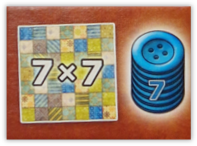
\includegraphics[width=0.18\textwidth]{res/pictures/assets/special-tile.png}
    % \vspace{-10pt}
    % Das folgende ist ein Trick, um "Abbilgung x.y" in eine
    % eigene Zeile zu packen. Der Text zwischen [ und ] steht
    % im Abbildungsverzeichnis. Der Text darunter wird
    % tatsächlich angezeigt.
    \caption[Sonderplättchen $7\times7$]{\unskip}
    Sonderplättchen $7\times7$
    \label{fig:special-tile}
\end{wrapfigure}

Bei dem Vorrat liegt das Sonderplättchen $7\times7$, in Abbildung \ref{fig:special-tile} zu sehen, welches der Spieler bekommt, der zuerst ein vollständig ausgefülltes $7\times7$-Quadrat aus Feldern auf seinem Ablageplan hat. Bei der Wertung am Ende des Spiels bringt dieses Sonderplättchen 7 Punkte. \cite{2014.PatchworkSpielanleitung}

Das Spiel endet, wenn die Zeitsteine der beiden Spieler das Zielfeld der Zeitleiste erreicht haben. Dabei verfallen überzählige Schritte und werden bei der Aktion \textbf{Vorrücken und Knöpfe erhalten} nicht ausgezahlt. \cite{2014.PatchworkSpielanleitung}

Zur Bestimmung des Gewinners müssen beide Spieler ihrer Knopfguthaben zählen, welches die Basis für ihren Punktestand darstellt. Falls das Sonderplättchen $7\times7$ ausgegeben wurde, wird dies auf den Punktestand des Spielers addiert. Vom Punktestand des Spielers werden nun für jedes freie Feld auf dem eigenen Ablageplan zwei Punkte abgezogen werden. Der Spieler mit der höchsten Gesamtpunktzahl ist Gewinner, bei Gleichstand gewinnt der Spieler, welcher zuerst das Zielfeld erreicht hat. \cite{2014.PatchworkSpielanleitung}

\subsection*{Ungenauigkeiten der Spielregeln}

In der Spielanleitung ist nicht genau beschrieben, was geschehen soll, wenn ein Spieler eine Spezialflicken legen muss, er jedoch auf seinem Ablageplan kein Feld mehr frei hat. Die Regel wird im Konsens so erweitert, dass falls dieser Fall eintrifft, der Spieler den Spezialflicken aus dem Spiel nimmt und neben sein Ablageplan legt. Auf die Wertung hat dies keinen Einfluss. \cite{2014.DiscussionSpecialPatch}

Außerdem wird in der Spielanleitung geschrieben, dass der Spieler, welcher \enquote{zuerst ein Quadrat von mindestens $7\times7$ Feldern auf seinem Ablageplan vollständig belegt hat} \cite{2014.PatchworkSpielanleitung}, das Sonderplättchen bekommt. Hier wird nicht ganz deutlich, wie genau diese Regel auszulegen ist. Die Regel wird im Konsens wie folgt interpretiert: Es muss kein vollständiges Quadrat ($8\times8$, $9\times9$) das $7\times7$-Quadrat umschließen, es reicht aus, wenn $7\times7$-Felder vollständig von Flicken bedeckt sind. Somit ist erlaubt, dass neben dem $7\times7$-Quadrat weitere Felder ausgefüllt sind und die gesamte Form auf dem Ablageplan kein Quadrat sein muss. \cite{2014.Discussion7x7}

\section{Spieltheoretische Analyse}

Patchwork ist ein \emph{sequentielles} 2\textendash{}Spieler\textendash{}Brettspiel. Sequentielle Spiele sind rundenbasierte Spiele, bei denen die Spieler nacheinander ziehen \cite[S. 53]{2014.GameTheoryThroughExamples}. Außerdem ist Patchwork ein Spiel mit \emph{perfekter Information}, \dash dass beide Spieler zu jeder Zeit genau wissen, was der andere Spieler getan hat und wie der jetzige Zustand des Spiels ist. Des Weiteren ist Patchwork ein \emph{Strategiespiel}. Wie für viele Strategiespiele typisch, enthält Patchwork auch keinen Zufall während des Spielablaufes. Die einzige Ausnahme ist vor dem Spielbeginn, da dort die Flicken in einer zufälligen Reihenfolge ausgelegt werden. Da beide Spieler in dem Brettspiel versuchen einen Sieg zu erreichen, handelt es sich weiterhin um ein \emph{Nullsummenspiel}. Bei Nullsummenspielen wird der Gewinn für einen Spieler als Verlust des anderen Spielers angesehen. Auch wenn das in Patchwork für einen einzelnen Spielzug nicht unbedingt der Fall sein muss, geht es bei Nullsummenspielen aber nur um das Gewinnen oder Verlieren des gesamten Spiels.

\subsection*{Anzahl der möglichen Startpositionen}

Das Brettspiel ist bis auf die Startposition der Spielteile deterministisch. Der einzige Zufallsfaktor beim Start ist das Auslegen der einzelnen Flicken im Kreis. Es gibt insgesamt 33 Flicken, welche ausgelegt werden müssen. Jedoch ist der kleinste Flicken, welcher nur 2 Felder auf einem Ablageplan einnimmt ($2\times1$ bzw. $1\times2$), immer an der gleichen Position direkt hinter der Spielfigur. Somit gibt es nur noch 32 Flicken, dessen Positionen angeordnet werden müssen. Eine solche Anordnug aller 32 Flicken auf 32 mögliche Positionen wird als \emph{Permutation} bezeichnet und besitzt $32! = 263.130.836.933.693.530.167.218.012.160.000.000$ Möglichkeiten. Somit gibt es $\approx 2{,}6 \cdot 10^{35}$ mögliche Startpositionen.

\subsection*{Isomorphie der Zeitpläne}

Wie bereits in »\nameref{section:spielregeln}« erläutert, existieren zwei verschiedene Zeitpläne, welche jedoch nur anders gestaltet sind. Somit sind beide Zeitpläne isomorph zueinander, \dash sie weisen dieselbe Struktur auf, obwohl der konkrete Aufbau verschieden ist. Diese innere Struktur ist zusammen mit den beiden Zeitplänen in \ref{tabelle:isomorphie-zeitplan} veranschaulicht.

\begin{table}[!ht]
    \centering
    \begin{tabular}[t]{cc}
        \adjustbox{center, width=0.4735\textwidth, valign=m, margin=0 1ex 0 0}{\begin{tikzpicture}
                                                                                       \node [inner sep=0pt,,outer sep=0pt,clip,rounded corners=0.15cm] (image) at (0,0) {\includegraphics[width=0.625\textwidth]{res/pictures/assets/time-board-side-1.png}};
                                                                                       \drawshadow{image}
                                                                                   \end{tikzpicture}} &
        \adjustbox{center, width=0.4735\textwidth, valign=m, margin=0 1ex 0 0}{\begin{tikzpicture}
                                                                                       \node [inner sep=0pt,,outer sep=0pt,clip,rounded corners=0.15cm] (image) at (0,0) {\includegraphics[width=0.625\textwidth]{res/pictures/assets/time-board-side-2.png}};
                                                                                       \drawshadow{image}
                                                                                   \end{tikzpicture}} \\
        \multicolumn{2}{c}{\adjustbox{valign=m, margin=0 2ex 0 2ex}{Zugrundeliegende Struktur des Zeitplans:}}                                                                            \\
        \multicolumn{2}{c}{\adjustbox{width=0.97\textwidth}{
\includegraphics{res/pictures/time-board-structure.pdf}}}                                                                     \\
    \end{tabular}
    \vspace{5pt}
    \caption{Die Zeitpläne zusammen mit der zugrundeliegenden Struktur}
    \label{tabelle:isomorphie-zeitplan}
\end{table}

Aus diesem Grund kann Patchwork nachfolgend als ein Spiel betrachtet werden, da die Auswahl eines konkreten Zeitplans keinen Unterschied für die Betrachtung ausmacht.

\subsection*{Länge des Spiels}
\label{subsection:analyse-laenge-des-spiels}

In der Spieltheorie ist der Begriff eines Spielzuges nicht eindeutig. Ein Spielzug könnte eine einzelne Aktion eines Spielers sein, \zB das Auswählen und Legen eines Flickens in Patchwork von einem Spieler. Jedoch kann ein Spielzug auch so verstanden werden, dass beide Spieler eine Aktion machen müssen. So wird beispielsweise in rundenbasierten Spielen wie Schach ein Spielzug oft so angesehen, dass einmal die weiße und einmal die schwarze Seite gezogen haben müssen. Aufgrund dieser Zweideutigkeit wird ein Spielzug in der Spieltheorie mit einem \hyperref[text:ply]{\emph{Ply}} genauer definiert.

\begin{defStrich}[Ply]
    Ein Spielzug, welcher von einem Spieler gezogen wird, und stellt die kleinste mögliche Aktion in einem Spiel dar. \cite[S. 213]{1959.GameTheoryStudiesCheckers}
\end{defStrich}
\label{text:ply}
\vspace{-0.2cm}

Durch diese Definition kann genau definiert werden, was mögliche \hyperref[text:ply]{\emph{Plys}} in Patchwork sind. Die obige Definition für einen Spielzug, bei dem beide Spieler gezogen haben müssen, ist in Patchwork sowieso schwierig umzusetzen, da ein Spieler mehrere \hyperref[text:ply]{\emph{Plys}} hintereinander ausführen kann. Insgesamt gibt es drei mögliche Arten von \hyperref[text:ply]{\emph{Plys}} in Patchwork:

\begin{itemize}
    \item Vorrücken des Zeitsteins und Knöpfe erhalten
    \item Einen Flicken nehmen und auf dem Ablageplan platzieren
    \item Das Legen eines Spezialflicken auf den Ablageplan
\end{itemize}

Immer wenn ein Spieler an der Reihe ist, kann er zwischen dem Vorrücken und dem Platzieren von drei Flicken unterscheiden. Die Aktion einen Spezialflicken auf die Decke zu legen, kommt im Spiel immer genau fünfmal vor.

Patchwork endet, sobald beide Zeitsteine der Spieler das Zielfeld auf der Zeitleiste erreicht haben. Um ein möglichst langes Spiel zu spielen, muss also die Anzahl der Felder, die ein Spieler mit seinem Zeitstein pro \hyperref[text:ply]{\emph{Ply}} vorzieht, minimiert werden.

Für die Aktion \enquote{Einen Flicken nehmen und auf der Decke platzieren} ist die Anzahl der Felder immer durch den ausgewählten Flicken vorgegeben und beträgt mindestens 1 und maximal 6 (vgl. Zeitkosten in Anhang \ref{anhang:section-patchwork-patches}).

\pagebreak

Die Anzahl der Felder bei der Aktion \enquote{Vorrücken des Zeitsteins und Knöpfe erhalten} ist abhängig von der relativen Position der einzelnen Zeitsteine zueinander. Die maximale Anzahl an Feldern, die ein Zeitstein in einem Zug vorrücken kann, beträgt 7. Da immer ein Spielerwechsel stattfindet, sobald der Zeitstein des derzeitigen Spielers weiter vorrangeschritten ist als der Zeitstein des Gegners, muss für eine maximale Anzahl die Distanz zwischen den Zeitsteinen möglichst groß sein. Ein Zeitstein kann sich von dem anderem Zeitstein nur um maximal 6 Felder entfernen. Das ist der Fall, wenn ein Flicken mit Zeitkosten 6 ausgewählt wird, während sich beide Zeitsteine auf demselben Feld befinden. Nach dieser Aktion ist der andere Spieler an der Reihe, welche sein Zeitstein um 7 Felder fortbewegen kann (Distanz von 6 Feldern $+$ 1 Feld, um weiter vorrangeschritten zu sein als der andere Zeitstein). Die minimale Anzahl an Felder bei der Vorrücken-Aktion beträgt 1 und kann bei drei Spielzuständen auftreten. Zuerst ist es möglich, dass beide Zeitsteine auf demselben Feld sind, sodass der Spieler, welcher an der Reihe ist, seinen Zeitstein nur 1 Feld vorrückt. Weiterhin ist es möglich, dass ein Zeitstein auf dem Feld vor dem Ziel ist, während der andere Spieler bereits im Ziel ist. In dieser Situation darf der Zeitstein auch nur um ein Feld vorgerückt werden. Zuletzt existiert noch die Situation am Spielanfang. Da hier auch beide Zeitsteine auf demselben Feld \textemdash{} dem Startfeld des Zeitplans \textemdash{} sind, darf der Startspieler den Zeitstein auch nur um ein Feld vorrücken.

Um die Länge des Spiels zu maximieren, sollte jeder Spieler so wenige Felder wie möglich vorrücken. Nutzt jeder Spieler immer die \enquote{Vorrücken des Zeitsteins und Knöpfe erhalten} Aktion, so gibt es insgesamt 54 \hyperref[text:ply]{\emph{Plys}}, da auf dem Zeitplan insgesamt 53 Felder sowie ein Start- und ein Zielfeld existieren. Während beim ersten und letzen \hyperref[text:ply]{\emph{Ply}} der Erste bzw. Zweite Spieler seinen Zeitstein nur um 1 Feld vorrückt, muss der Zeitstein während des Spiels immer 2 Felder vorgerückt werden, da die vorherige Aktion \textemdash{} auch eine \enquote{Vorrücken des Zeitsteins und Knöpfe erhalten} Aktion \textemdash{} impliziert, dass der Zeitstein des Gegners genau 1 Feld vor dem eigenen Zeitstein liegt. Die Zeitkosten bei der Aktion \enquote{Einen Flicken nehmen und auf der Decke platzieren} sind immer fest, wobei es insgesamt neun Flicken gibt, bei denen die Zeitkosten auch 2 betragen. So können optimal 9 Vorrücken-Aktionen durch die Auswahl dieser Flicken ersetzt werden. Weiterhin gibt es aber auch noch die vier in \ref{tabelle:flicken-mit-zeitkosten-1} dargestellten Flicken, welche nur Zeitkosten von 1 besitzen. Wird nun ein Vorrücken-\hyperref[text:ply]{\emph{Ply}} mit 2 Zeitkosten durch eine Kombination aus Flicken mit Zeitkosten 1 auswählen und auf der Decke Platzieren und anschließend ein Vorrücken-\hyperref[text:ply]{\emph{Ply}} mit Zeitkosten 1 ersetzt, ist das Spiel um 4 weitere \hyperref[text:ply]{\emph{Plys}} verlängert.

\begin{table}[!ht]
    \centering
    \resizebox{\textwidth}{!}{
        \begin{tabular}[t]{c|c|c|c}
            \adjustbox{valign=t, raise=-16.25ex}{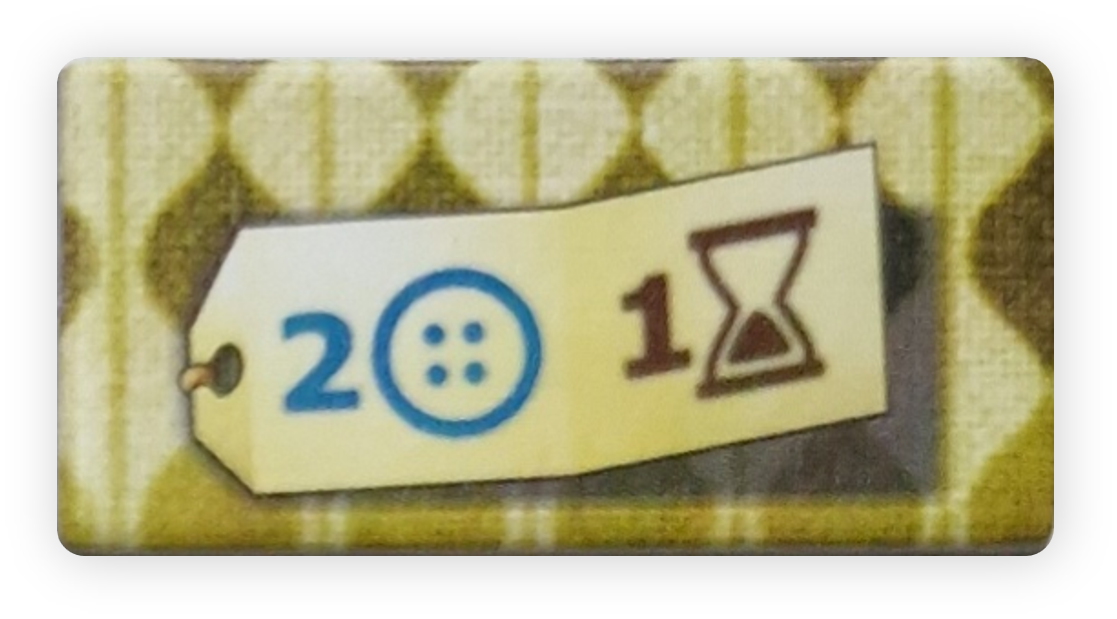
\includegraphics[width=0.2\textwidth]{res/pictures/assets/00-front.png}} &
            \adjustbox{valign=t, raise=0ex}{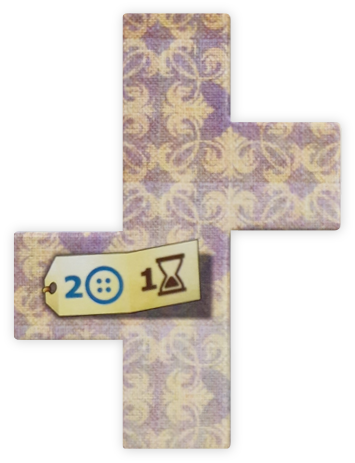
\includegraphics[width=0.3\textwidth]{res/pictures/assets/06-front.png}}      &
            \adjustbox{valign=t, raise=-9.05ex}{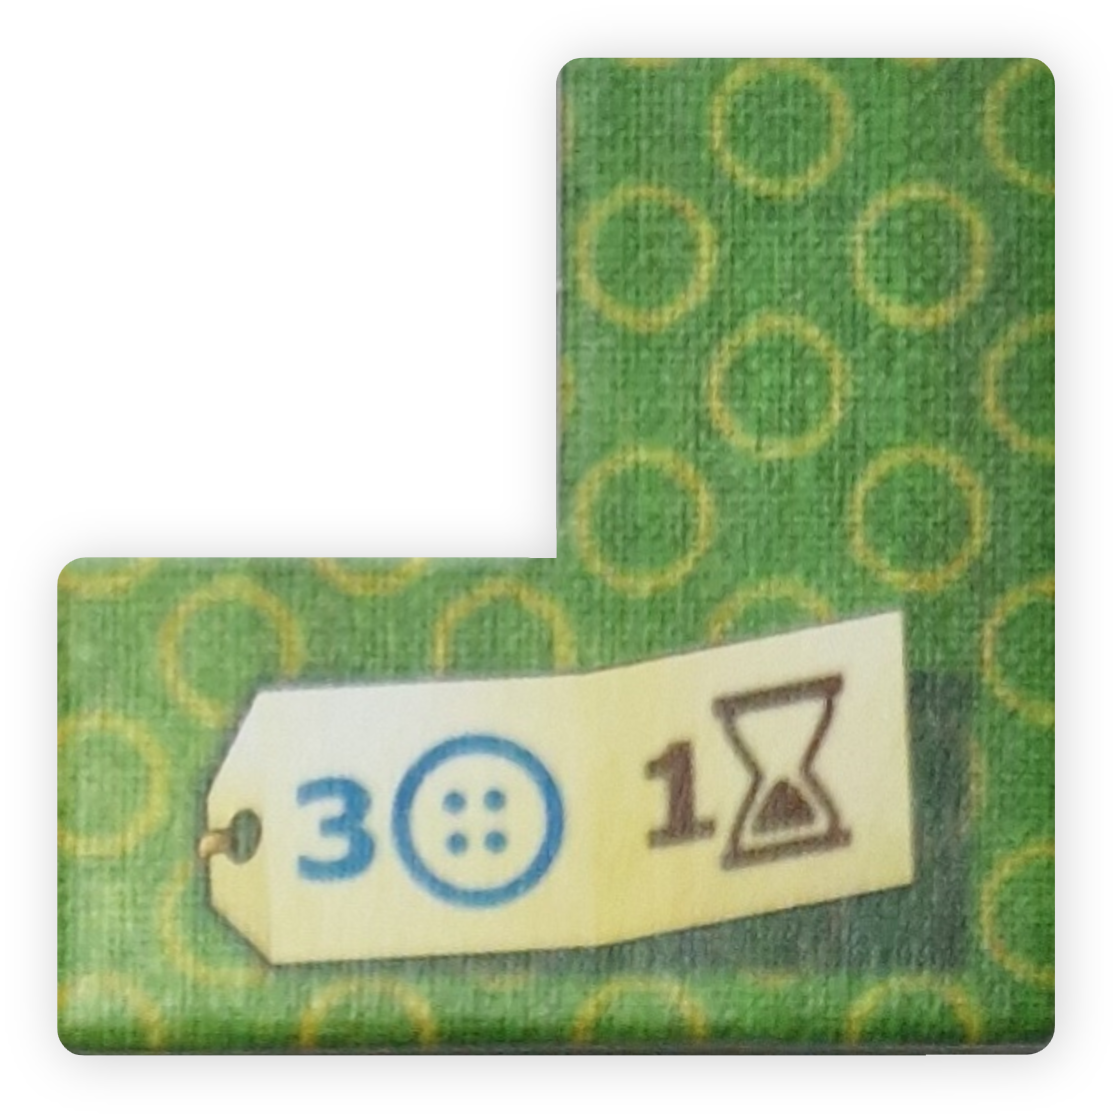
\includegraphics[width=0.2\textwidth]{res/pictures/assets/21-front.png}}  &
            \adjustbox{valign=t, raise=-16.25ex}{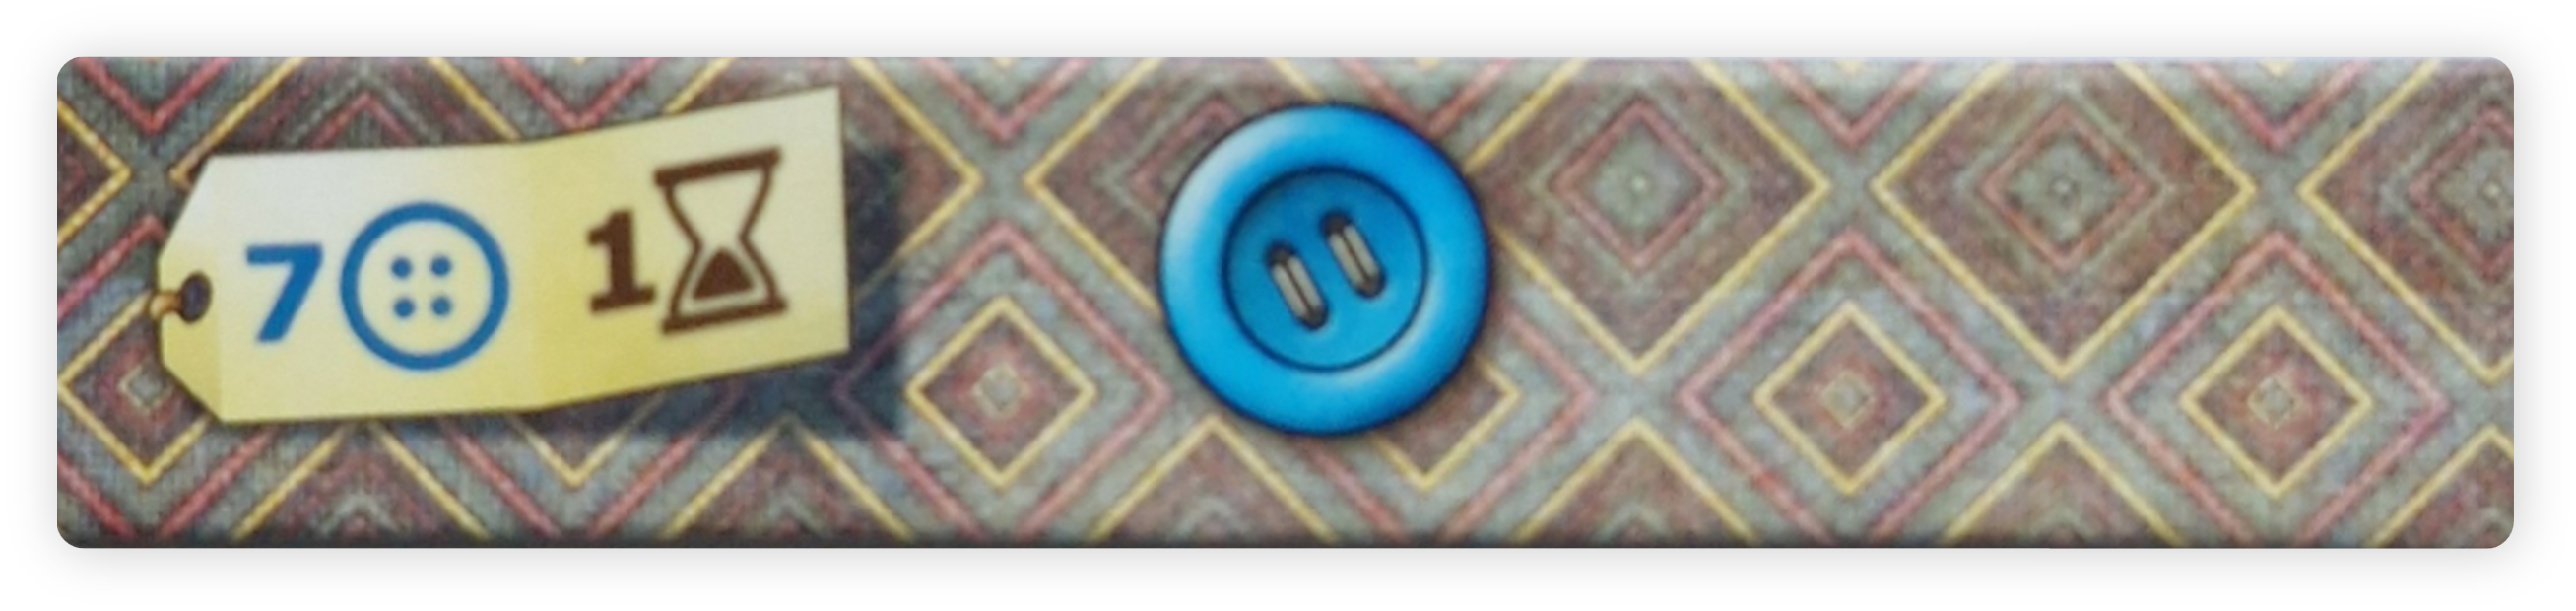
\includegraphics[width=0.5\textwidth]{res/pictures/assets/27-front.png}}   \\
        \end{tabular}
    }
    \vspace{5pt}
    \caption{Die vier Flicken mit Zeitkosten 1}
    \label{tabelle:flicken-mit-zeitkosten-1}
    \vspace*{-0.35cm}
\end{table}

Das ist möglich, da wie oben beschrieben der Zeitstein des derzeitigen Spielers immer direkt hinter dem Zeitstein des Gegners ist. Wird nun ein Flicken mit Zeitkosten 1 ausgewählt, befindet sich der Zeitstein des derzeitigen Spielers auf dem Zeitstein des Gegners. So kann ein Vorrücken-\hyperref[text:ply]{\emph{Ply}} mit Zeitkosten von 1 anstatt 2 ausgeführt werden. Da alle anderen Flicken höhere Zeitkosten verlangen, ist keine weitere Optimierung des Spiels hinsichtlich der der maximalen Länge mehr möglich.

Die maximale Länge des Brettspiels ergibt sich somit aus der Kombination der 54 Vorrücken-\hyperref[text:ply]{\emph{Plys}} zusammen mit den 4 zusätzlich gewonnenen \hyperref[text:ply]{\emph{Plys}} durch das Legen von Flicken mit Zeitkosten 1. Weiterhin kommen noch die fünf \hyperref[text:ply]{\emph{Plys}} für das Legen von Spezialflicken hinzu. Somit beträgt die maximale Länge von Patchwork \textbf{63} \hyperref[text:ply]{\emph{Plys}}.

\subsection*{Maximale Anzahl aufeinanderfolgender \hyperref[text:ply]{Plys} eines Spielers}

Neben der Gesamtlänge des Spiels kann auch betrachtet werden, wie oft ein Spieler maximal hintereinander ziehen kann. Wie oben erläutert, kann der Zeitstein des Gegners maximal 6 Felder vor dem eigenen Zeitstein liegen. Zuerst können in 4 \hyperref[text:ply]{Plys} die vier Flicken mit Zeitkosten 1 genommen und platziert werden. Danach kann noch ein Flicken mit Zeitkosten 2 erworben werden, sodass sich der Zeitstein auf demselben Feld wie der Gegner befindet. In einem weiteren \hyperref[text:ply]{Ply} kann der Spieler noch durch laufen bzw. Flicken platzieren an dem Gegner vorbeiziehen. Zuletzt ist es möglich, dass der Spieler dabei einen Spezialflicken passiert und diesen in einem weiteren \hyperref[text:ply]{Ply} legen muss\footnote{Da der Spieler maximal 6 Felder auf dem Zeitplan auf einmal vorrücken kann, ist es nicht möglich 2 Spezialflicken zu passieren, da diese auch immer genau 6 Felder voneinander entfernt sind.}. Somit kann ein Spieler maximal \textbf{7} \hyperref[text:ply]{Plys} hintereinander ausführen.

\subsection*{Minimum und Maximum für die Anzahl an möglichen Aktionen}

Um die Komplexität von Patchwork zu untersuchen, ist es auch interessant zu betrachten, wie viele Auswahlmöglichkeiten einem Spieler bei seinem Zug zur Verfügung stehen.

Ist ein Spieler am Zug, kann er immer die Aktion \enquote{Vorrücken des Zeitsteins und Knöpfe erhalten} auswählen. Somit beträgt die minimale Anzahl an Aktionen mindestens 1. Dabei handelt es sich auch um das Minimum, da der derzeitige Spieler weniger Knöpfe in seinem Vorrat haben kann, als jede der ersten 3 Flicken nach der Spielfigur an Knöpfen kostet. Somit kann der Spieler sich keinen der Flicken leisten und muss automatisch seinen Zeitstein vorrücken.

Eine obere Schranke für die maximal mögliche Anzahl an Aktionen ergibt sich als:

\vspace*{-0.45cm}
\begin{equation}
    \text{Obere Schranke}_{\text{Aktionen}} = \:
    \underset{\mathclap{\substack{\rotatebox[origin=c]{90}{\(\{ \)} \mathstrut \\ \text{Vorrücken}}}}{1}
    + \:
    \overset{\mathclap{\substack{\text{maximale Auswahlanzahl} \mathstrut \\ \text{Flicken} \mathstrut \\ \rotatebox[origin=c]{-90}{\(\{ \)}}}}{3} \:
    \times \:
    \max\limits_{\mathclap{\substack{\phantom{\text{\tiny m}} \\ f\, \in\, \text{Flicken}}}} \:\,
    \left\lvert\, \text{Platziermöglichkeiten}\left( f \right)\, \right\rvert
\end{equation}
\vspace*{-0.15cm}

Dabei ist eine $+1$ für die Aktion \enquote{Vorrücken des Zeitsteins und Knöpfe erhalten} vorhanden. Weiterhin gibt es für einen Spieler die Möglichkeit aus maximal 3 Flicken einen Flicken auszuwählen. Diese Anzahl wird multipliziert mit der maximalen Anzahl an Möglichkeiten, mit dem ein Flicken auf dem Ablageplatz platziert werden kann.

Um die maximale Anzahl an Platzierungsmöglichkeiten festzulegen, muss zuerst betrachtet werden, auf wie viele Arten ein Flicken auf die Ablagedecke gelegt werden kann. Die Operationen, welche vor dem Platzieren auf einen Flicken angewendet werden können, sind Drehungen und Spiegelungen, wodurch die Flicken identisch zur Diedergruppe $D_4$ sind. Die Gruppe besteht aus 8 Elementen \cite[S. 33]{2015.AbstractAlgebra}, was somit gleichzeigt die maximale Anzahl an Transformationen für ein Flicken ist. Jedoch muss beachtet werden, dass die Flicken die maximale Anzahl nicht erreichen müssen. Zum Beispiel existiert ein $2\times2$ Flicken, welcher im Sinne der Diedergruppe 8 Ausprägungen besitzt, jedoch auf der Ablagedecke mit allen Drehungen und Spiegelungen immer genau dieselben Felder bedeckt. Für die maximale Platzierungsanzahl ist aber nur relevant, dass ein Flicken existiert, welcher bei allen 8 Transformationen eine andere Anordnung aufweist. Dieser Flicken existiert und ist in Abbildung \ref{fig:diedergruppe} dargestellt.

\pagebreak

\vspace*{-0.85cm}
\begin{figure}[!ht]
    \centering
    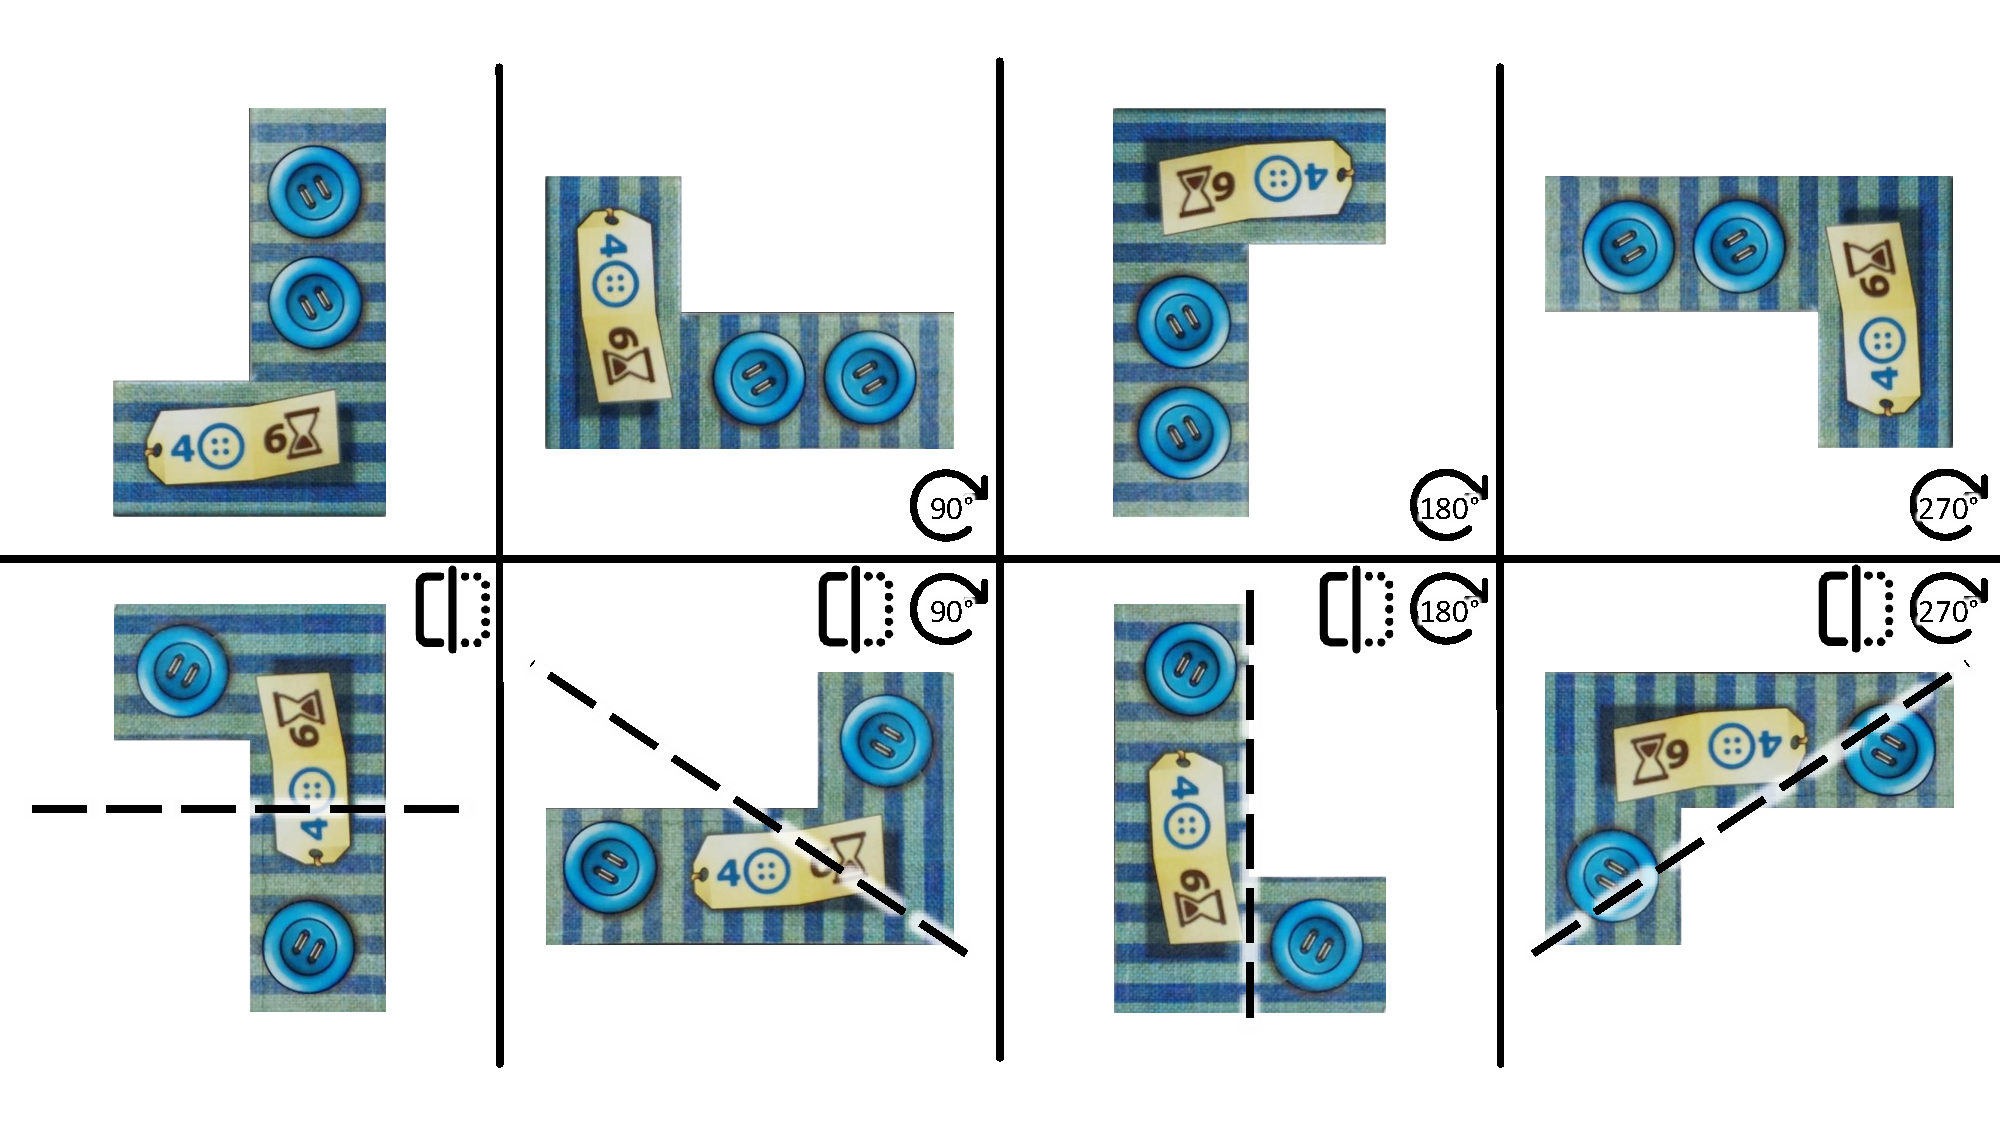
\includegraphics[width=0.835\textwidth]{res/pictures/dihedral-group.png}
    \vspace*{-0.23cm}
    \caption{Flicken mit 8 verschiedenen Transformationen}
    \label{fig:diedergruppe}
    \vspace*{-0.22cm}
\end{figure}

Weiterhin gibt es verschiedene Möglichkeiten den transformierten Flicken auf den $9\times9$ Felder großen Ablageplan zu legen. Die Möglichkeiten lassen sich dabei einfach wie in Term \ref{eqn:ablagefeld-platzierungen} in Abhängigkeit von der Breite und Höhe des Flickens sowie der Anzahl der unterschiedlichen Transformationen berechnen.

\vspace*{-0.28cm}
\vspace*{-0.4cm}
\begin{equation}
    \label{eqn:ablagefeld-platzierungen}
    \left( 9 - \text{Höhe}  + 1 \right) \cdot
    \left( 9 - \text{Breite} + 1 \right) \cdot
    \left\lvert\, \text{Transformationen} \,\right\rvert
    \vspace*{-0.28cm}
\end{equation}

Die Anzahl der Platzierungsmöglichkeiten für den in \ref{fig:diedergruppe} dargestellten $3\times 2$ großen Flicken beträgt somit $\left( 9 - 3 + 1 \right) \cdot \left( 9 - 2 + 1 \right) \cdot 8 = 448$. Jedoch muss für die Platzierungsmöglichkeiten beachtet werden, dass sich die Anzahl reduziert, je größer ein Flicken ist. Somit muss für alle Flicken, dessen Höhe $\le 3$ und Breite $\le 2$ ist \textemdash{} wobei mindestens eine der beiden Ungleichungen strikt (also $<$) sein muss \textemdash{} überprüft werden, ob mehr Platzierungsmöglichkeiten bestehen als bei dem Flicken von \ref{fig:diedergruppe}. Es existieren nur 3 Flicken dieser Art, welche in Tabelle \ref{tabelle:kleine-flicken} dargestellt sind. Jeder dieser Flicken weißt dabei durch die geringere Anzahl an verschiedenen Transformationsmöglichkeiten insgesamt weniger Platzierungsmöglichkeiten auf als der Flicken in \ref{fig:diedergruppe}.

\vspace*{-0.35cm}
\begin{table}[!ht]
    \centering
    \begin{tabular}[t]{c|c|c|c}
        \raisebox{0pt}[0.35ex][0.35ex]{Flicken} & \adjustbox{valign=m}{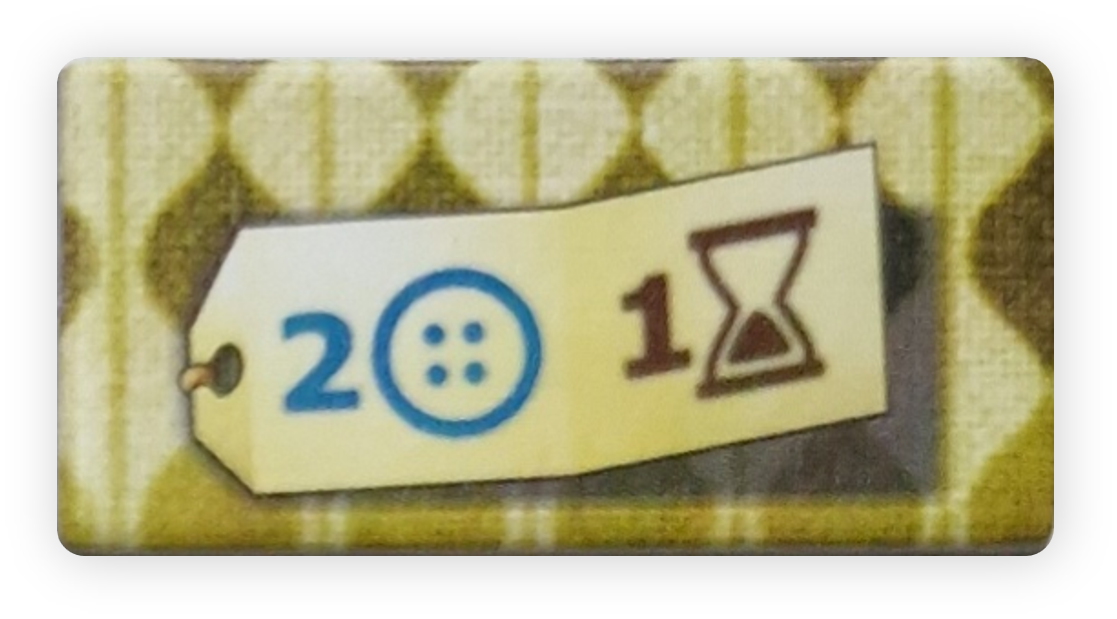
\includegraphics[width=0.1525\textwidth]{res/pictures/assets/00-front.png}} & \adjustbox{valign=m}{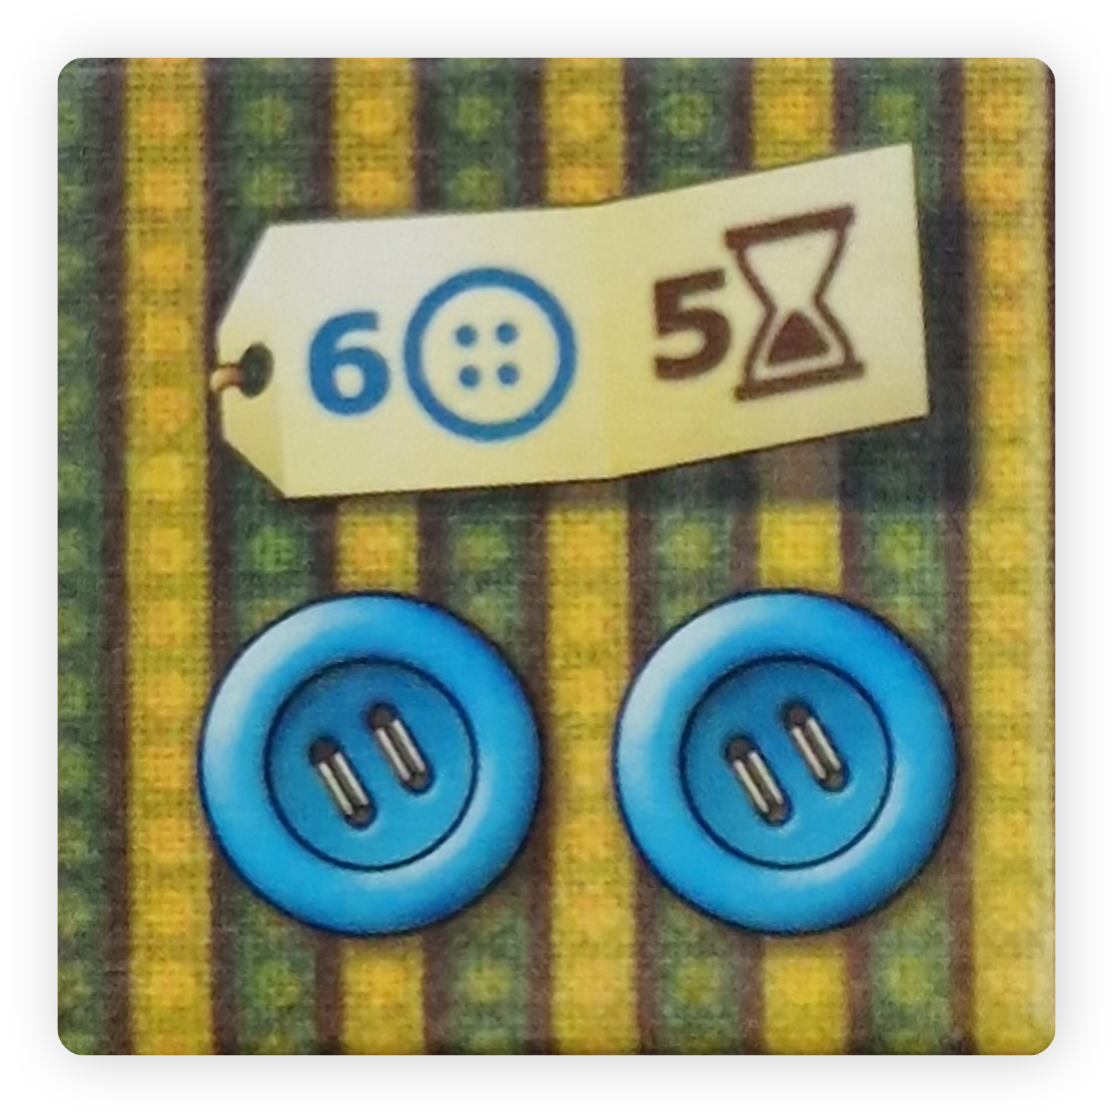
\includegraphics[width=0.1525\textwidth]{res/pictures/assets/09-front.png}} & \adjustbox{valign=m}{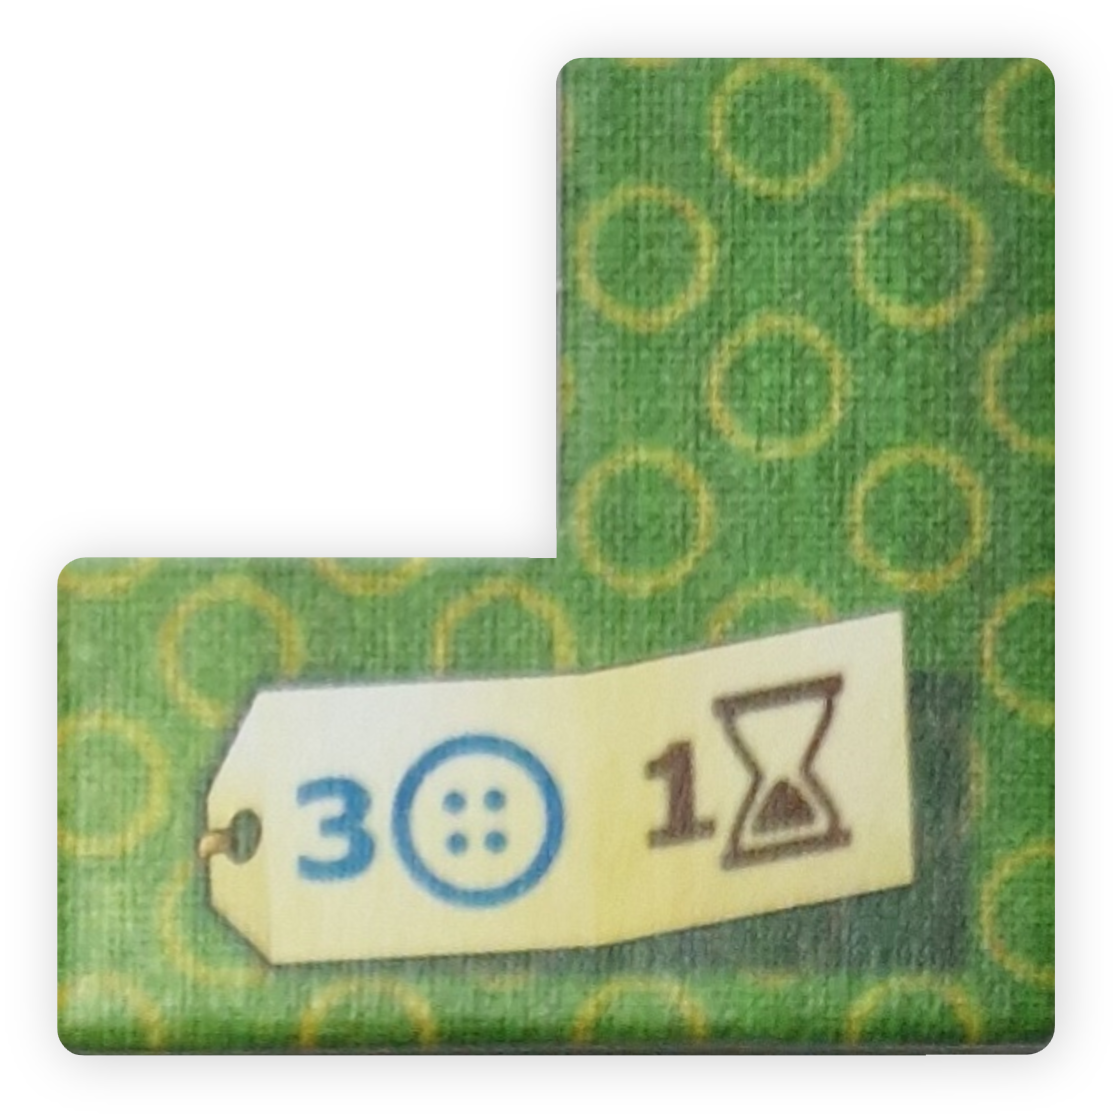
\includegraphics[width=0.1525\textwidth]{res/pictures/assets/21-front.png}} \\ \hline
        \makecell{Platzierungs-                                                                                                                                                                                                                                                                                                                       \\möglichkeiten} & $9 \cdot 8 \cdot 2 = 144$                                                                      & $8 \cdot 8 \cdot 1 = 64$                                                                       & $8 \cdot 8 \cdot 4 = 256$                                                                      \\
    \end{tabular}
    \vspace{2pt}
    \caption{Platzierungsmöglichkeiten der kleineren Flicken}
    \label{tabelle:kleine-flicken}
\end{table}
\vspace*{-4.5cm}

\pagebreak

\begin{wrapfigure}{r}{0.25\textwidth}
    \vspace*{-0.1cm}
    \centering
    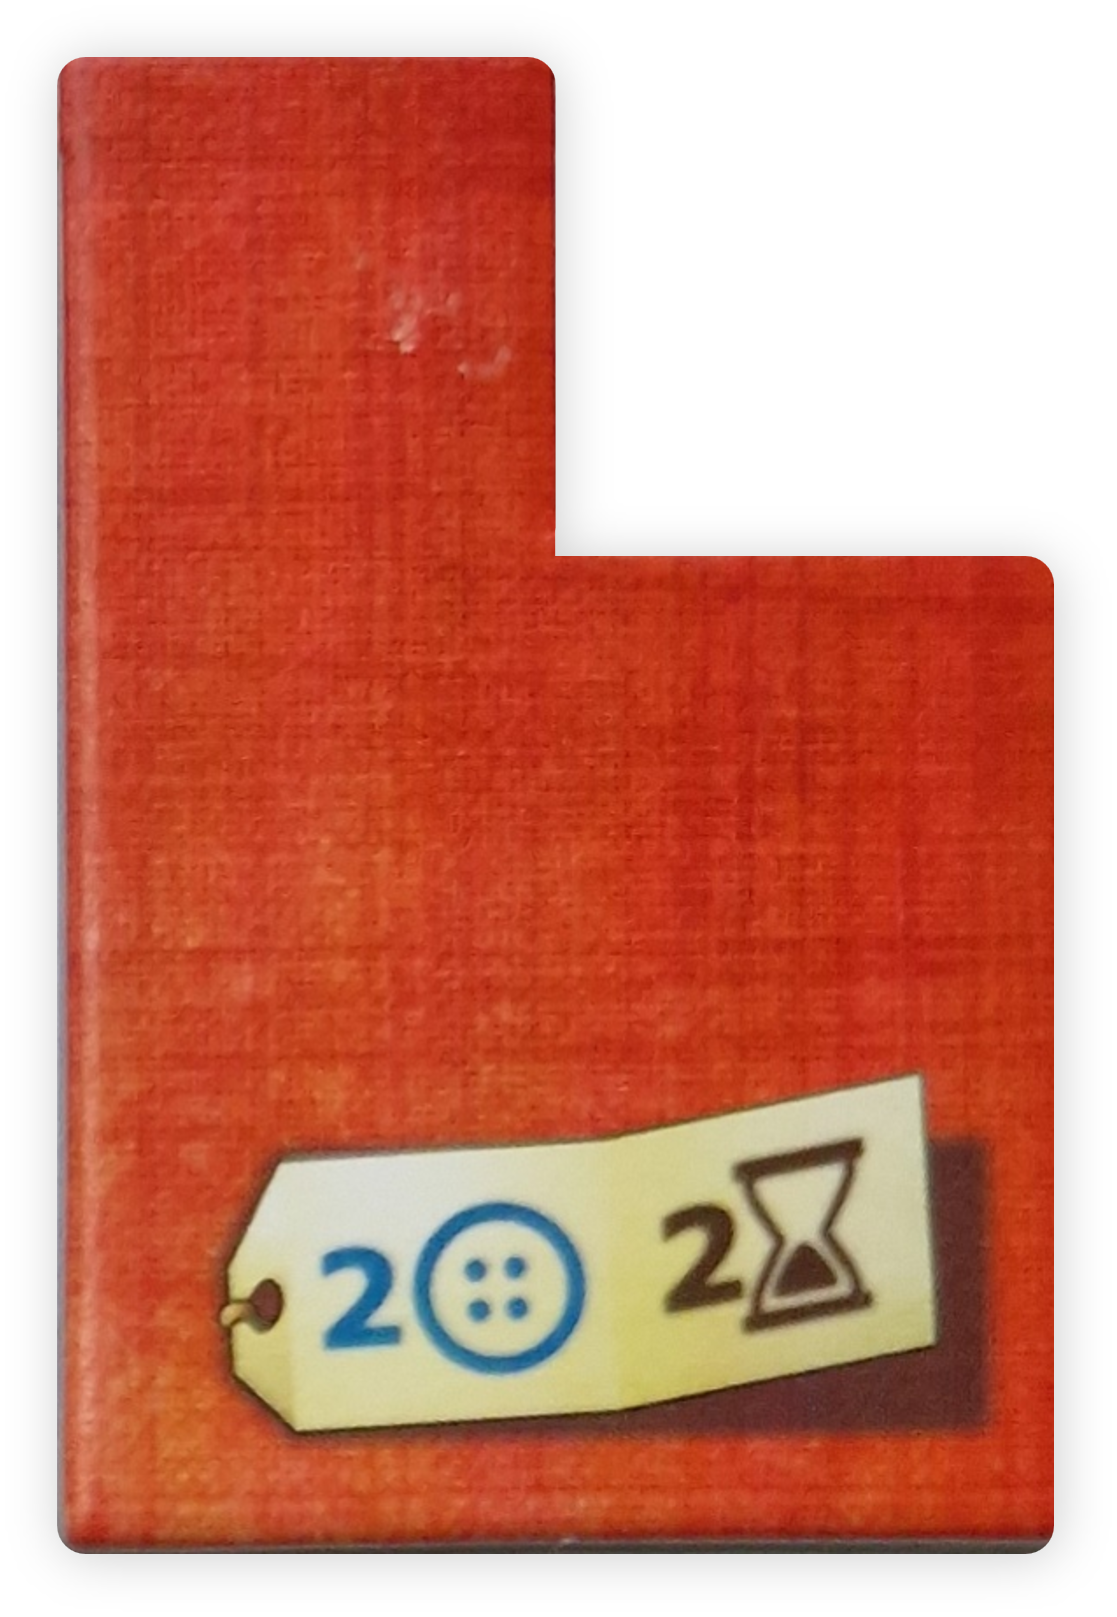
\includegraphics[width=0.12\textwidth]{res/pictures/assets/08-front.png}

    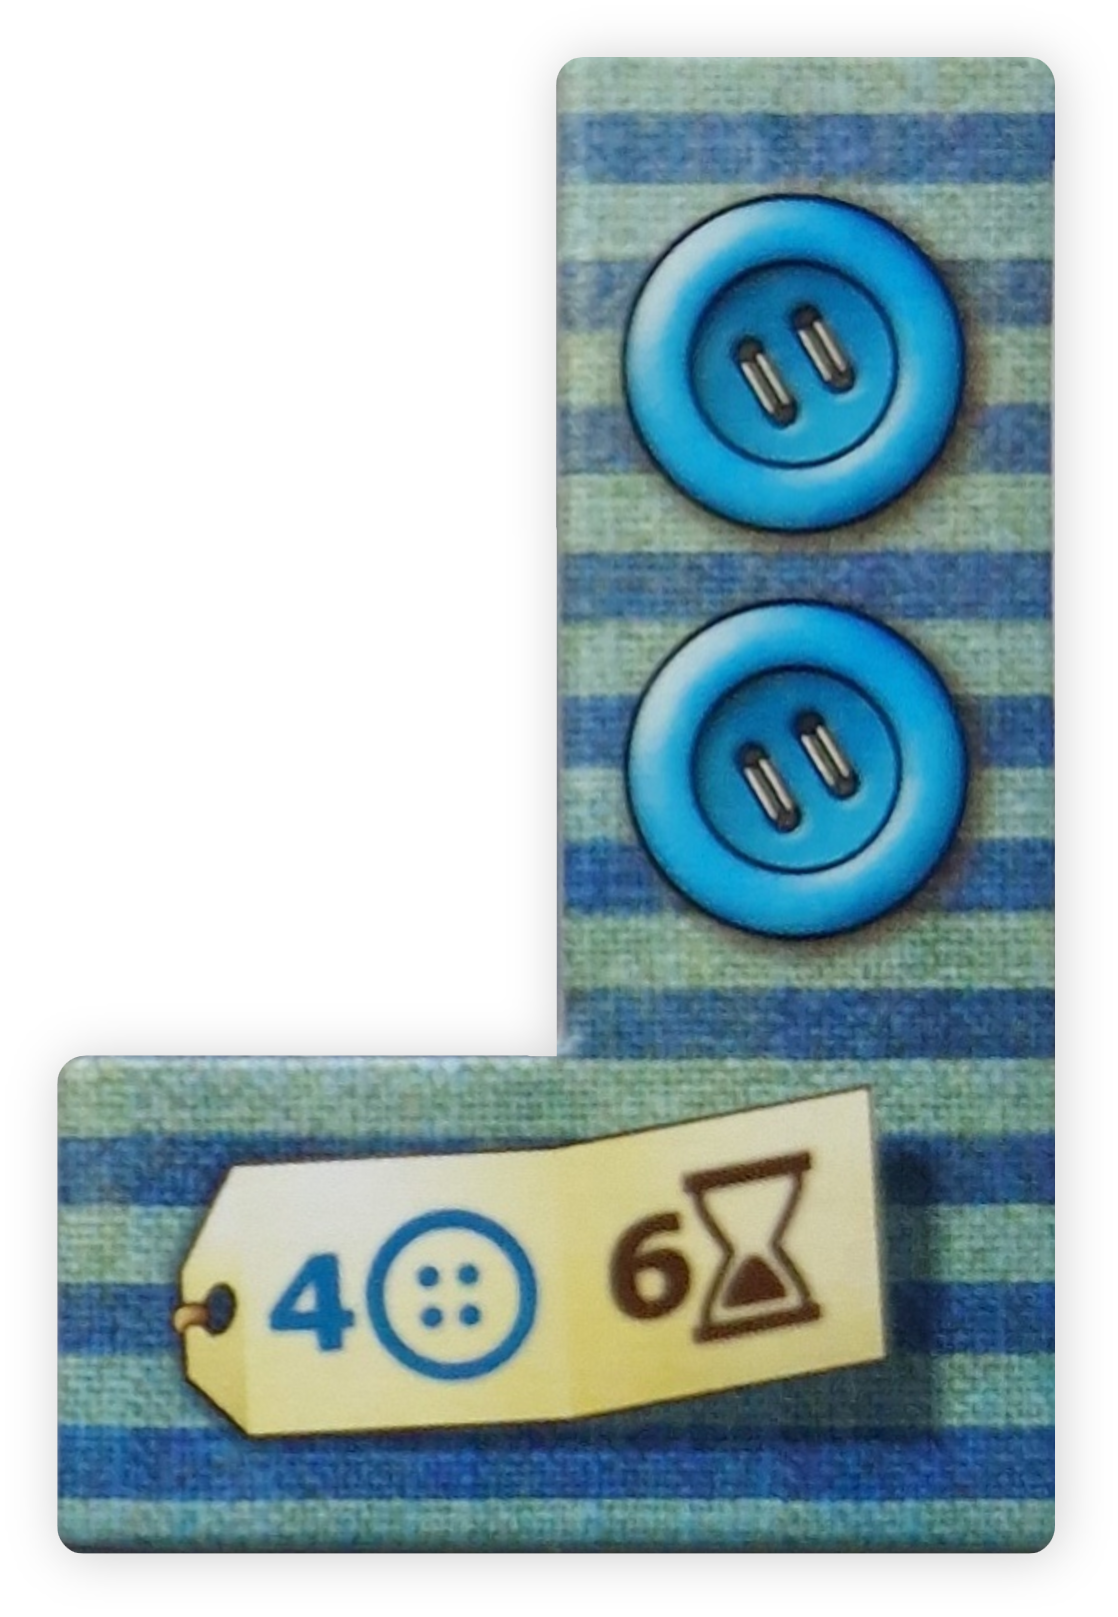
\includegraphics[width=0.12\textwidth]{res/pictures/assets/14-front.png}

    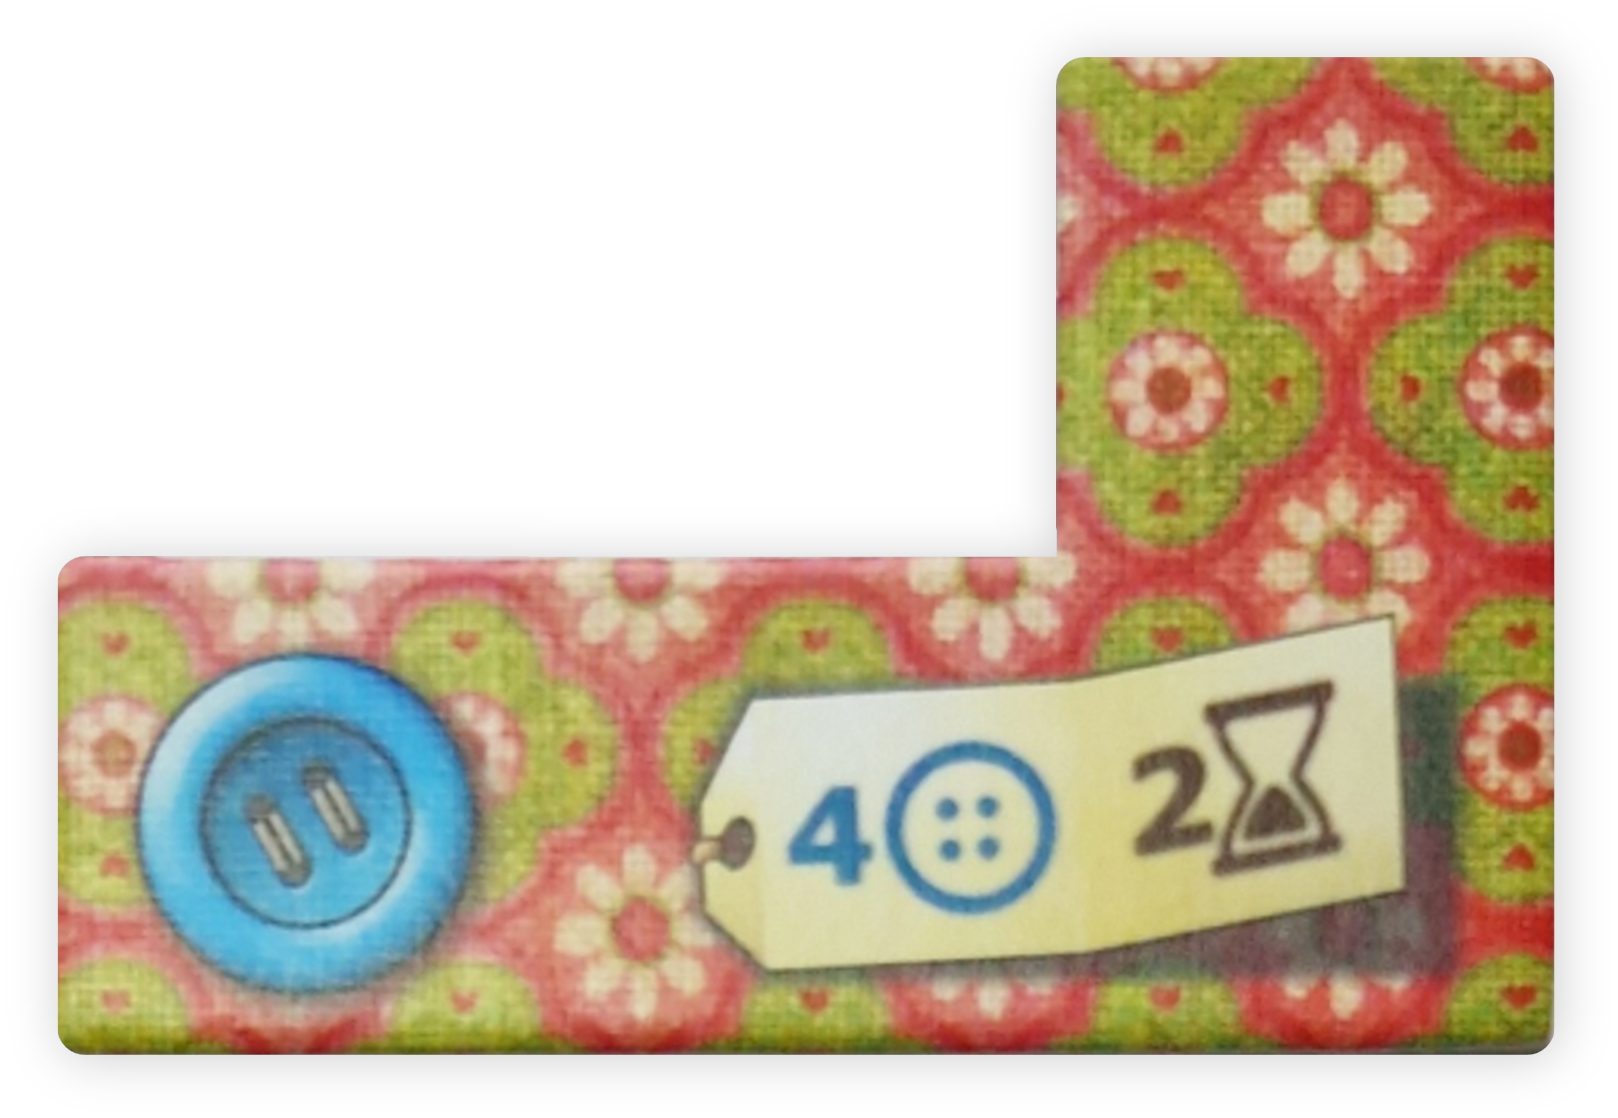
\includegraphics[width=0.18\textwidth]{res/pictures/assets/19-front.png}
    % \vspace{-10pt}
    % Das folgende ist ein Trick, um "Abbilgung x.y" in eine
    % eigene Zeile zu packen. Der Text zwischen [ und ] steht
    % im Abbildungsverzeichnis. Der Text darunter wird
    % tatsächlich angezeigt.
    \caption[Alle Flicken mit 448 Platzierungsmöglichkeiten]{\unskip}
    Alle Flicken mit 448 Platzierungsmöglichkeiten
    \label{fig:flicken-mit-448}
    \vspace*{-0.1cm}
\end{wrapfigure}

Um sicherzustellen, dass die maximale Platzierungsmöglichkeit auf dem Ablageplan auch tatsächlich für die drei zur Verfügung stehenden Flicken auftreten kann, müssen mindestens drei unterschiedliche Flicken mit einer Größe von $3 \times 2$ bzw. $2 \times 3$ existieren, welche 448 Möglichkeiten zur Platzierung auf dem Ablageplan besitzen. Das ist der Fall, wie die Flicken in Abbildung \ref{fig:flicken-mit-448} zeigen.

Um die maximale Anzahl an möglichen Aktionen festzustellen, muss zuletzt noch das Platzieren von Spezialflicken als Sonderfall betrachtet werden. Da alle Spezialflicken eine Größe von $1 \times 1$ besitzen, unterscheiden sich die Transformationen nicht hinsichtlich der Platzierung auf dem Ablageplan. Somit gibt es $9 \cdot 9 \cdot 1 = 81$ mögliche Aktionen einen Spezialflicken auf dem Ablageplan zu platzieren.

Das tatsächliche Maximum für die mögliche Anzahl an Aktionen ergibt sich dann als das Maximum der normalen Aktionen und der Aktion \enquote{Legen eines Spezialflicken} wie in \ref{eqn:max-aktionen} dargestellt ist:

\vspace*{-0.4cm}
\begin{equation}
    \label{eqn:max-aktionen}
    \text{Maximum}_{\text{Aktionen}} = \max \left\{ 1 + 3 \cdot 448\, ,\, 81 \right\} = 1345
\end{equation}

Dabei ist anzumerken, dass die maximale Anzahl an Platzierungsmöglichkeiten für normale sowie Spezialflicken nur genau dann möglich ist, wenn der Ablageplan noch leer ist. Weiterhin kann die maximale Auswahlmöglichkeit auch bereits direkt am Anfang des Spiels geschehen, da alle Flicken in \ref{fig:flicken-mit-448} mit dem Startbudget von 5 Knöpfen gekauft werden können.

\subsection*{Obere und untere Schranke für die Wertung eines Spielers}

In dieser Sektion wird eine obere und eine untere Schranke für die Wertung eines Spielers am Ende des Spiels festgesetzt. Da sich die Wertung aus dem am Ende vorhandenen Vorrat an Knopf-Plättchen und der Anzahl der Lücken im eigenen Spielbrett zusammensetzt, werden zunächst die maximal möglichen Werte für diese beiden Komponenten bestimmt. Anschließend werden die Schranken für die Wertung eines Spielers am Ende des Spiels festgesetzt.

% Reference for this paragraph: /code/patchwork/transposition_table/src/zobrist_hash.rs

Ein Spieler hat 2 Möglichkeiten bei der Wertung möglichst viele positive Punkte zu sammeln. Erstens kann der Spieler das $7 \times 7$ Sonderplättchen erhalten, was die Wertung um 7 Punkte erhöht. Weiterhin zählt jeder Knopf in seinem Vorrat einen Punkt. Zu Beginn erhält jeder Spieler 5 Knöpfe. Der Knopfvorrat kann nur durch die 9 Knopf-Wertungen auf der Zeitleiste erhöht werden. Dabei ist die Erhöhung des Knopfvorrates abhängig von den Flicken auf dem Ablageplan. Da der Ablageplan eine feste Größe besitzt, existiert somit auch eine Obergrenze für das zusätzliche Knopfeinkommen und die Anzahl der positiven Punkte für die Wertung ist von oben begrenzt. Die einfache Obergrenze für den positiven Anteil bei der Endbewertung ist daher $5+7+81\cdot 9=741$.

Diese Obergrenze würde aber erfordern, dass alle Flicken auf dem Ablageplan mindestens die gleiche Anzahl an Knopfeinkommen haben, wie die Anzahl der Felder, die sie bedecken. Diese Annahme gilt für keinen der Flicken in Patchwork. Für eine realistischere Obergrenze werden alle Flicken nach dem prozentualen Anteil des Knöpfeinkommens im Verhältnis zur Anzahl der Felder, die sie bedecken, sortiert (Siehe Anhang \ref{anhang:section-patchwork-patches}). Werden nun alle Flicken ausgewählt, bis die Grenze von 81 kombinierten Feldern erreicht ist, ergibt sich eine neue Obergrenze für das maximale Knopfeinkommen durch den Ablageplan von 32. Eine beispielhafte Anordnung dieser Flicken ist in Abbildung \ref{fig:quilt-board-max-button-income} zu sehen. Dabei bleiben 2 Felder auf dem Ablageplan frei. Jedoch können alle Flicken mit 2 oder weniger Feldern kein Knopfeinkommen generieren, wodurch dies kein Problem darstellt.

\begin{figure}[!ht]
    \centering
    \begin{minipage}{.48\textwidth}
        \centering
        \begin{tikzpicture}
            \node [inner sep=0pt,,outer sep=0pt,clip,rounded corners=0.15cm] (image) at (0,0) {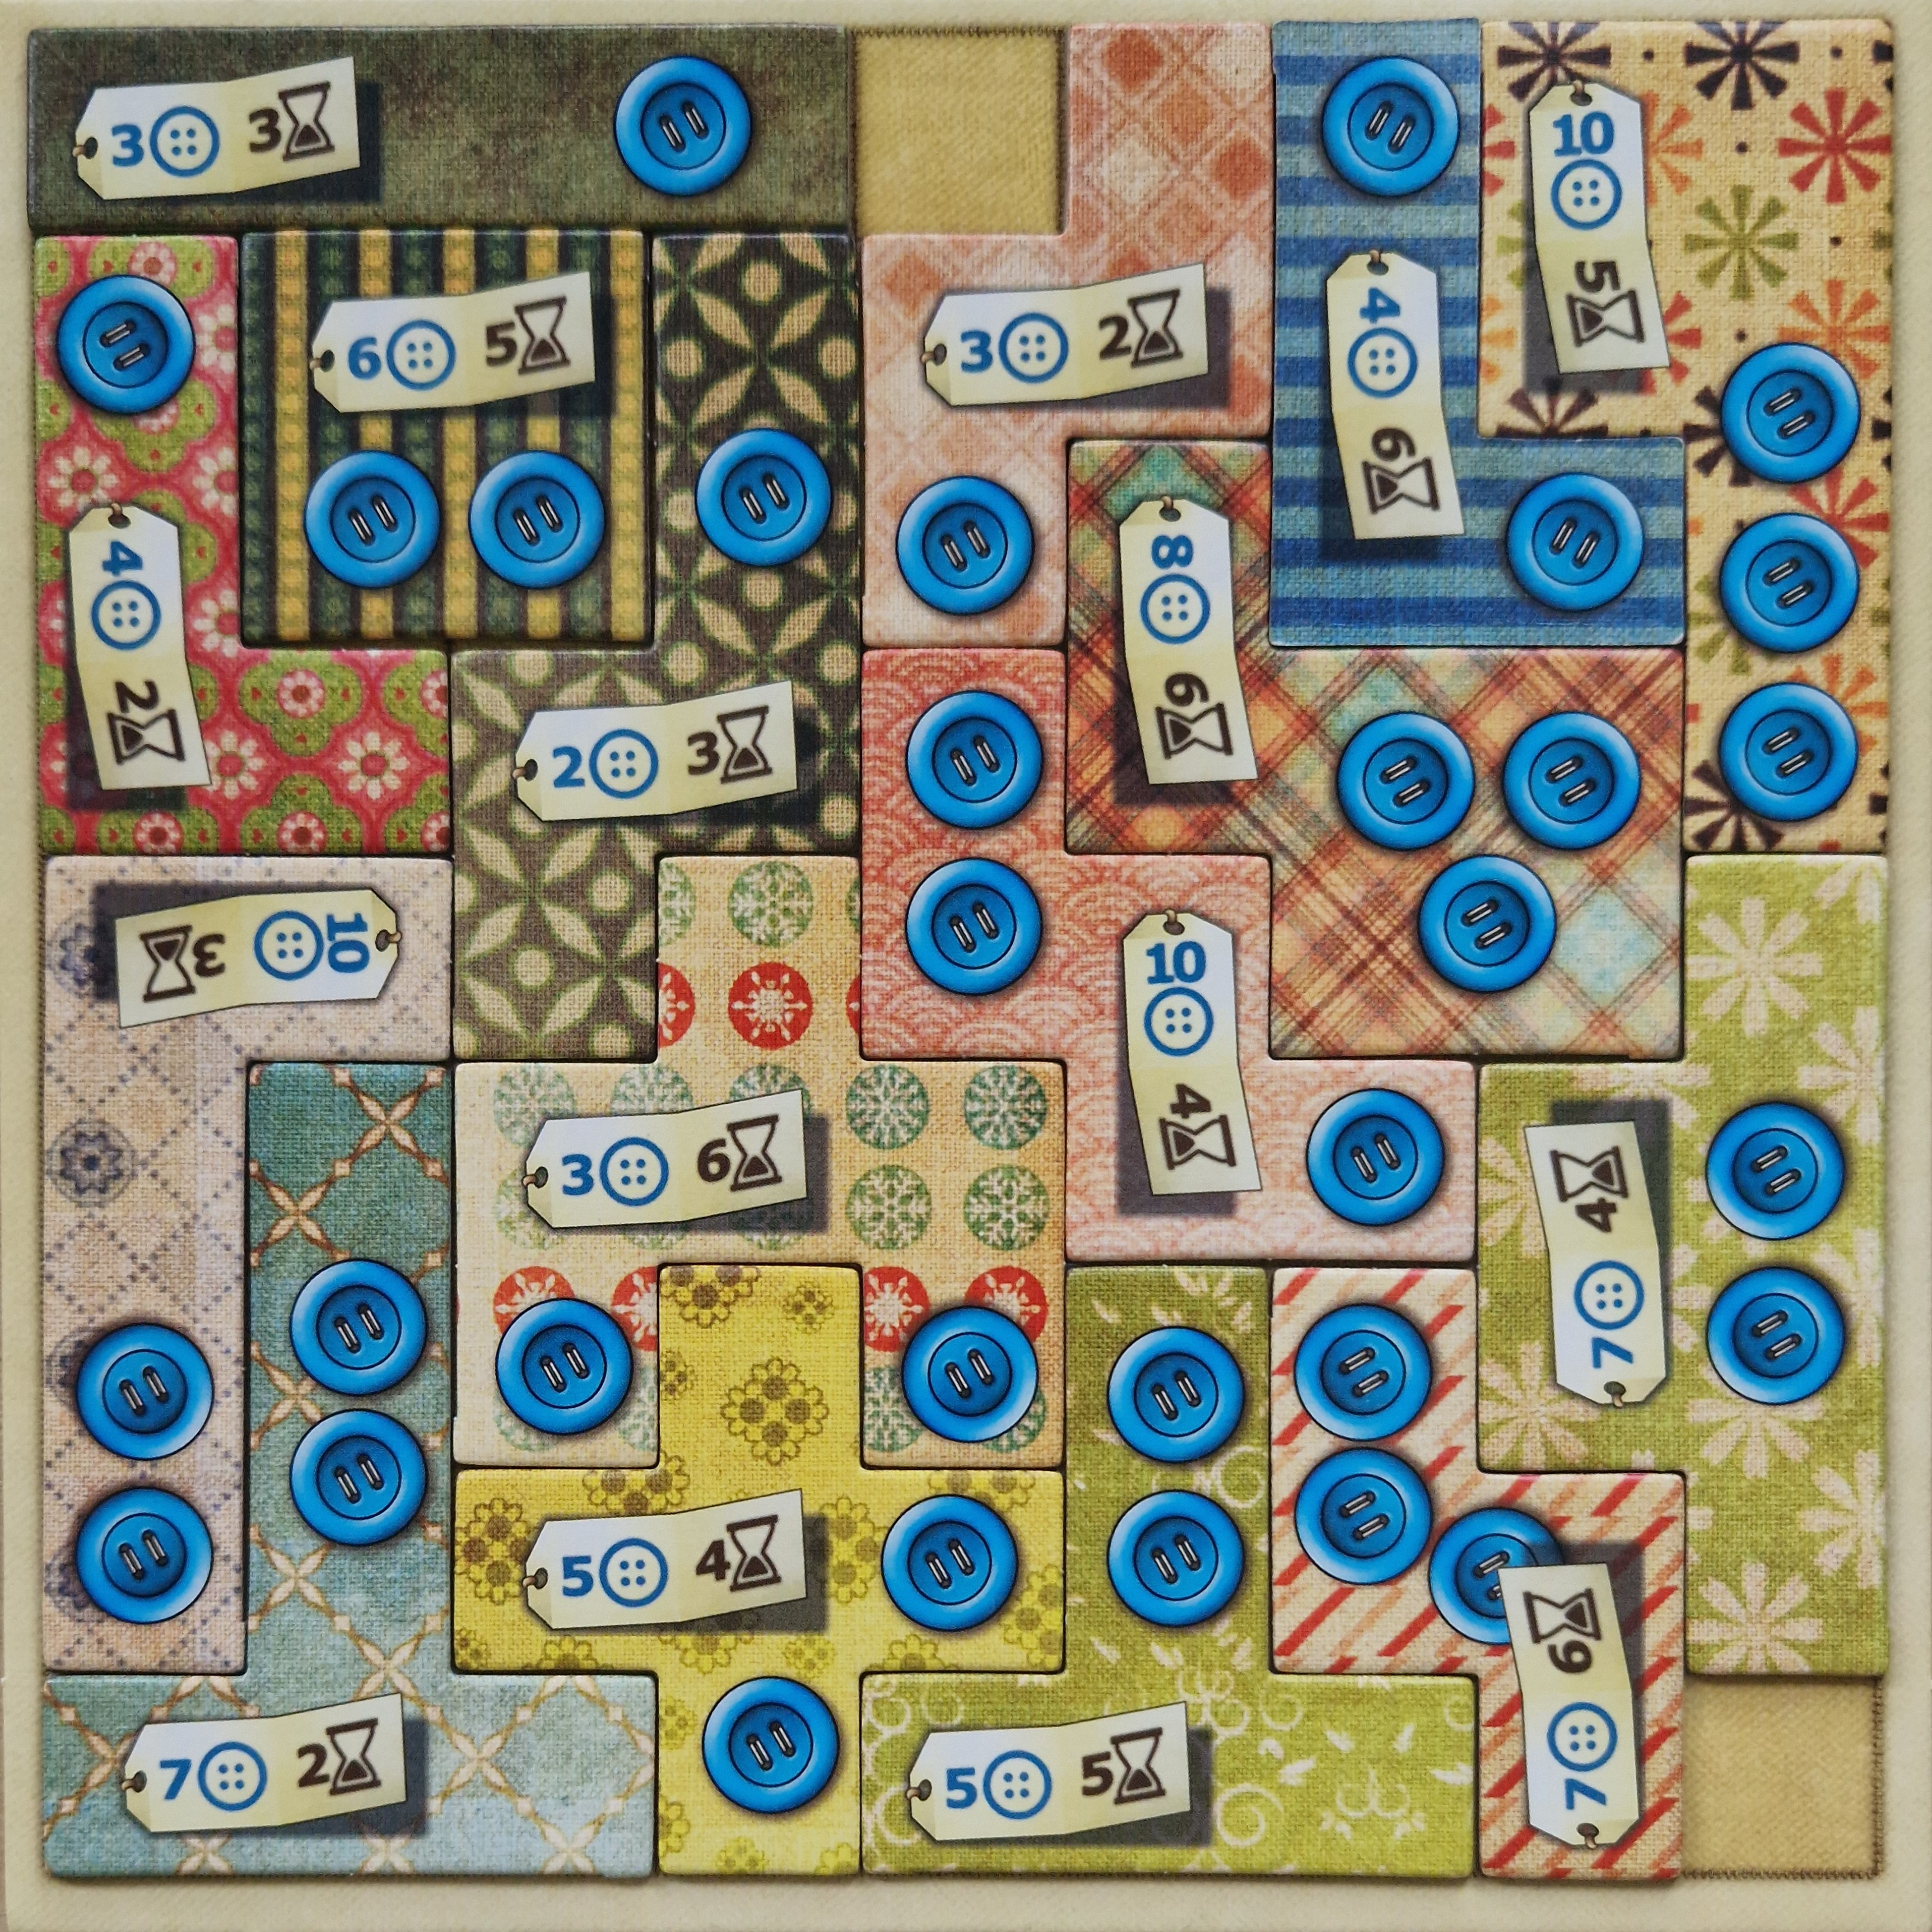
\includegraphics[width=0.765\linewidth]{res/pictures/max-button-income.jpg}};
            \drawshadow{image}
        \end{tikzpicture}
        \captionsetup{format=plain, singlelinecheck=false}
        \setcapindent{0pt}
        \caption{Anordnung von Flicken mit einem Knopfeinkommen von 32 \\ \phantom{und Zeitkosten von 66}}
        \label{fig:quilt-board-max-button-income}
    \end{minipage}
    \hfill
    \begin{minipage}{.48\textwidth}
        \centering
        \begin{tikzpicture}
            \node [inner sep=0pt,,outer sep=0pt,clip,rounded corners=0.15cm] (image) at (0,0) {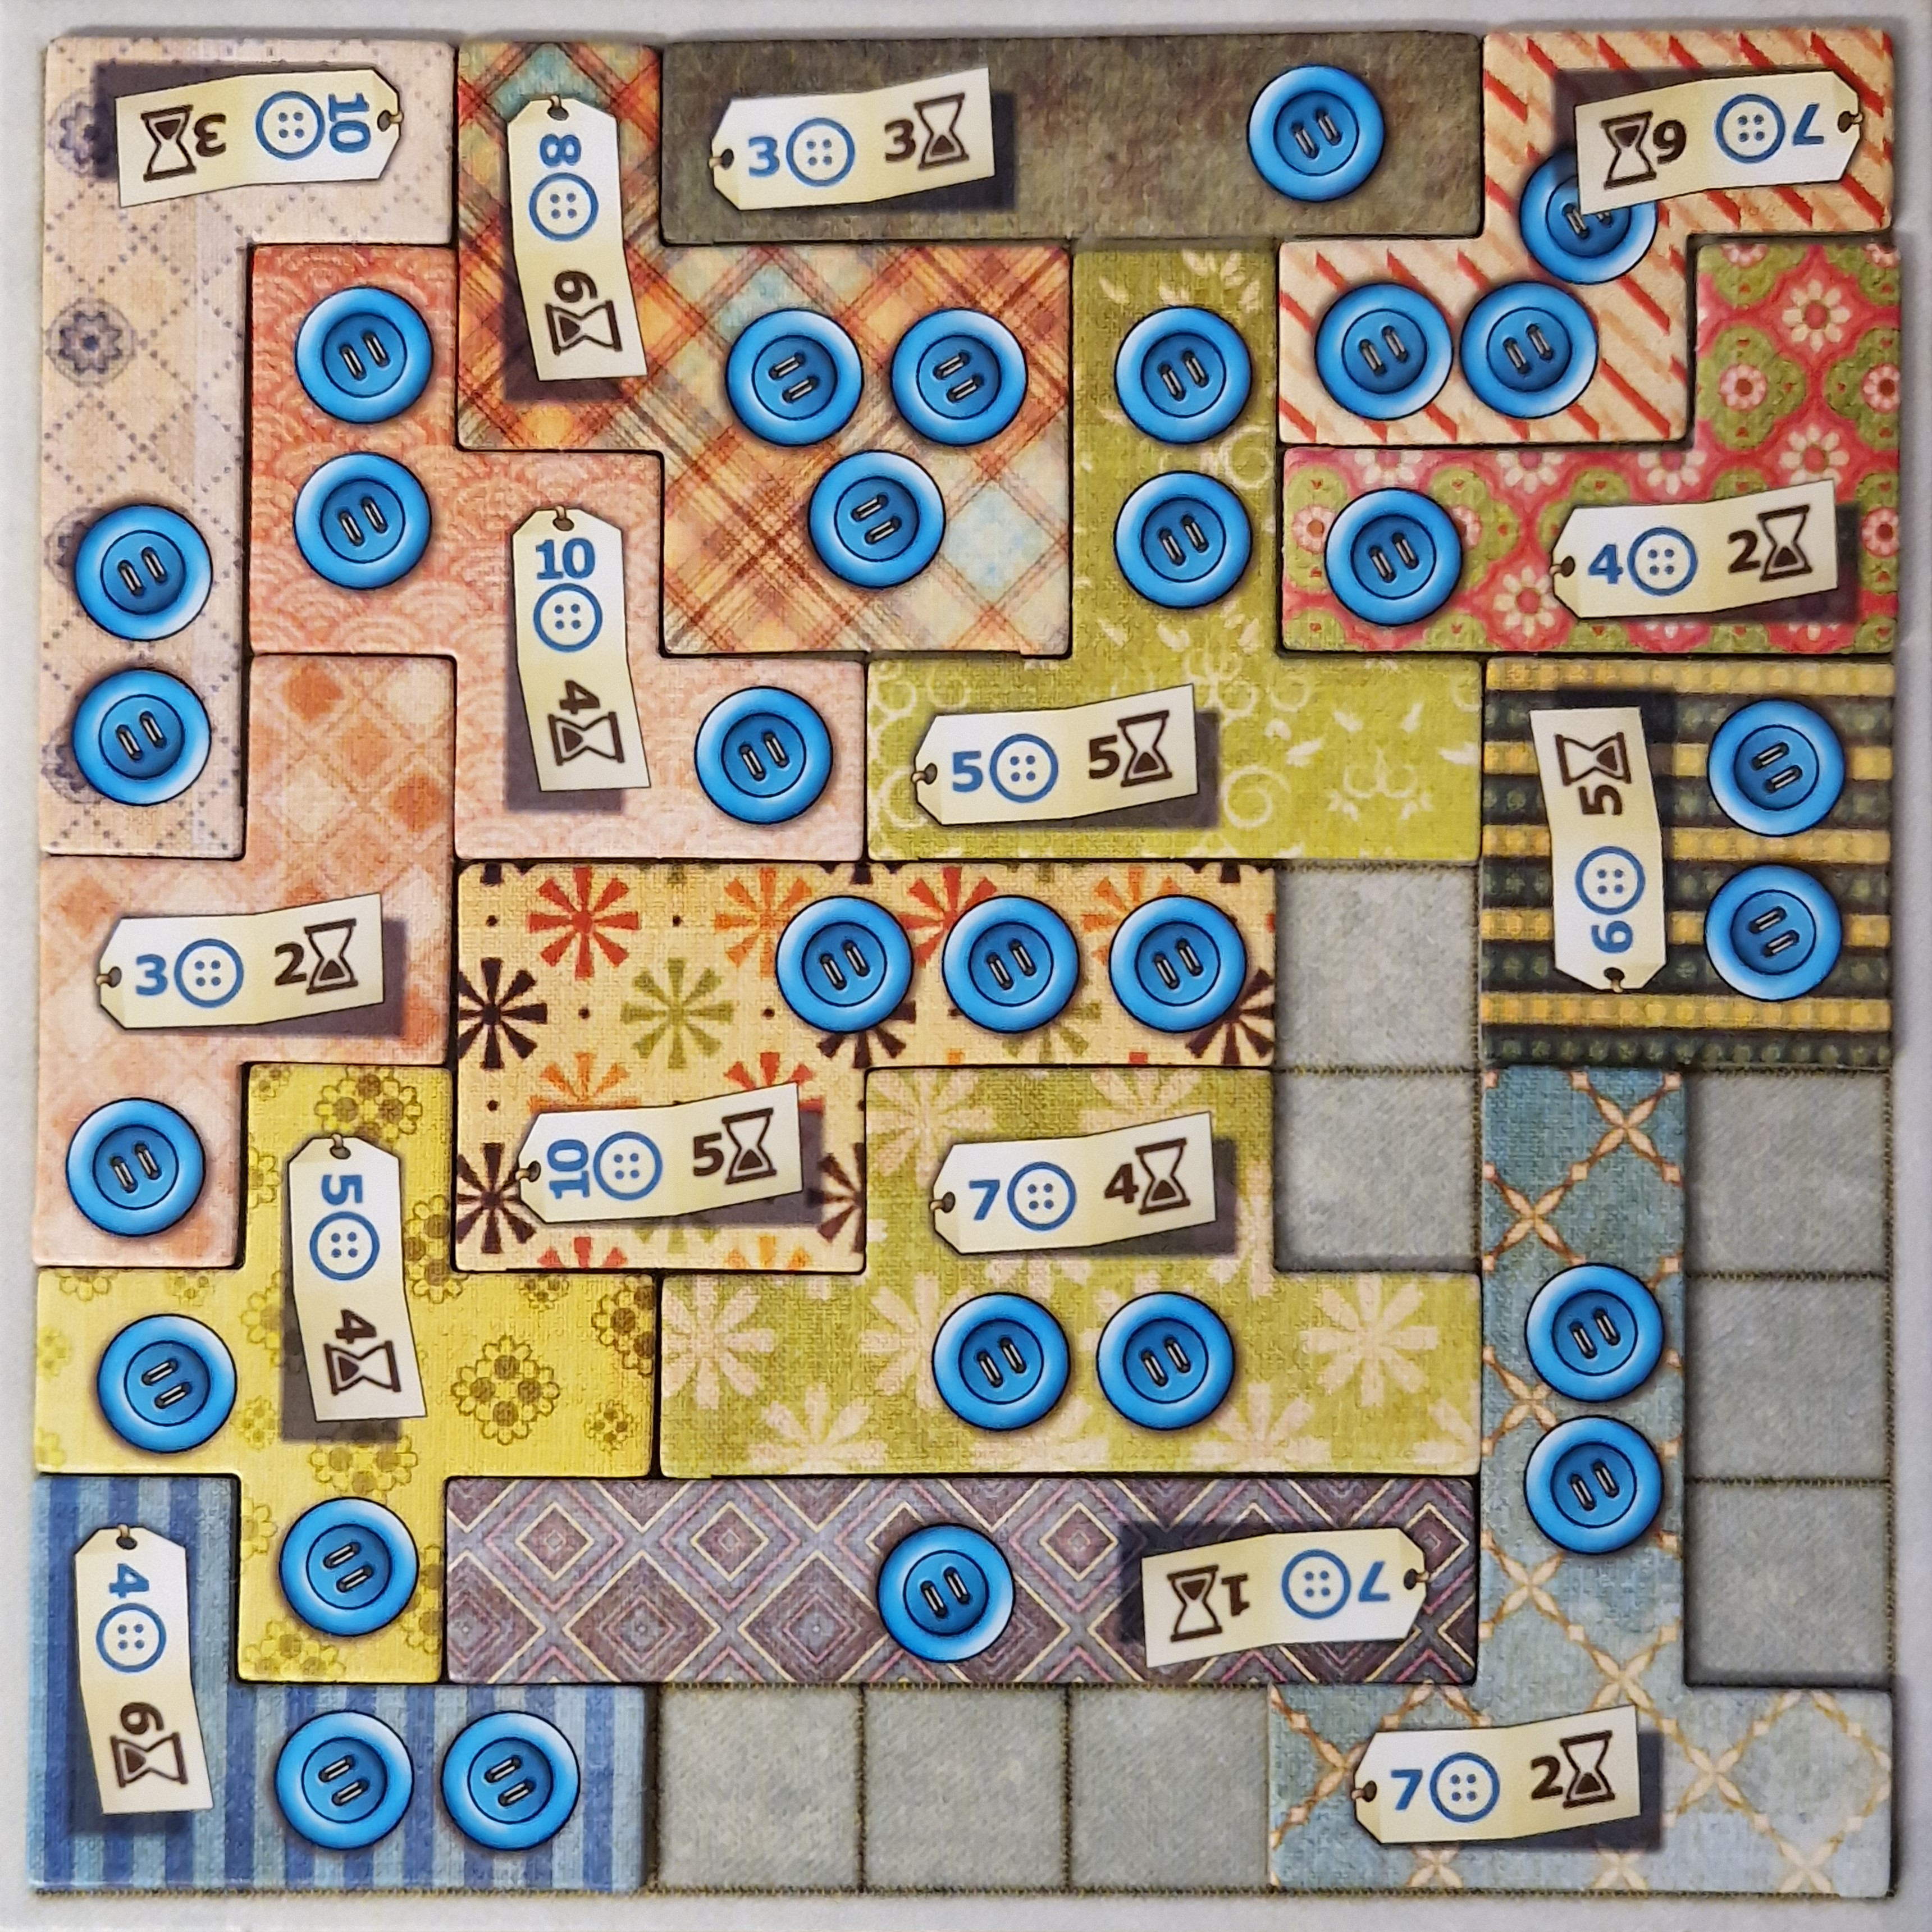
\includegraphics[width=0.765\linewidth]{res/pictures/real-max-button-income.jpg}};
            \drawshadow{image}
        \end{tikzpicture}
        \captionsetup{format=plain, singlelinecheck=false}
        \setcapindent{0pt}
        \caption{Anordnung von Flicken mit einem Knopfeinkommen von 30 \\ und Zeitkosten von 58}
        \label{fig:quilt-board-real-max-button-income}
    \end{minipage}
\end{figure}

Jedoch betragen die benötigten Zeitkosten bei dieser Anordnung $66$, wodurch diese Anordnung im tatsächlichen Spiel nicht auftreten kann. Aus diesem Grund muss für die Bewertung eines Flickens noch die benötigte Zeit wie in Term \ref{eqn:patch-value-for-max-button-income} einfließen.

\begin{equation}
    \label{eqn:patch-value-for-max-button-income}
    \frac{\text{Knopfeinkommen}}{\text{Felder}\, \cdot\, \text{Zeitkosten}}
\end{equation}

Somit ergibt sich eine neue Sortierung und Anordnung der Flicken auf dem Ablageplan, wie in Abbildung \ref{fig:quilt-board-real-max-button-income}. Das maximale Knopfeinkommen beträgt dabei $30$ Knöpfe und die benötigte Zeit beträgt $58$. Auf dem Zeitplan selbst, existieren nur $54$ Felder. Ein Spieler kann aber auf dem letzten Feld vor dem Ziel noch einen Flicken nehmen und läuft \emph{immer genau $1$} Feld. Somit kann der Spieler hier auch ein Flicken mit den maximalen Zeitkosten von $6$ nehmen. Da $58 - 6 = 52 < 54$ ist die Anordnung in \ref{fig:quilt-board-real-max-button-income} also auch tatsächlich während des Spiels erreichbar. Eine obere Schranke für das Knopfeinkommen durch den Ablageplan im gesamten Spiel ist somit die Anzahl der Knopf-Wertungen auf dem Zeitplan ($9$) multipliziert mit dem maximalen Knopfeinkommen pro Knopf-Wertung ($30$) $= 270$.

Der Spieler bekommt bei der Wertung am Ende nur Punkte abgezogen, wenn nicht alle Felder auf seinem Ablageplan bedeckt sind. Es gibt mehrere Möglichkeiten solch einen vollen Ablageplan im Spielverlauf zu erhalten (ein Beispiel hierfür ist in Anhang \ref{anhang:section-ablageplan-81} zu sehen). Somit kann für eine Obergrenze bei der Wertung mit einem Punktabzug von 0 gerechnet werden. Zusammen mit dem Ablageplan von \ref{fig:quilt-board-real-max-button-income} würde sich somit mit $5 + 7 + 30 \cdot 9 - 0 = \boldsymbol{282}$ eine neue Obergrenze für die maximale Wertung eines Spielers ergeben.

Nun kann sich der minimal erreichbaren Wertung eines Spielers zugewendet werden. Eine sehr einfache Untergrenze für die minimale Wertung eines Spielers ist $-162$, \dash ein leerer Ablageplan und 0 Knöpfe im Knopfvorrat. Diese Wertung kann jedoch offensichtlich nicht erreicht werden, da die einzige Möglichkeit Knöpfe aus dem Vorrat abzugeben gleichzeitig darin besteht, den Ablageplan zu füllen und jeder Spieler mit mindestens 5 Knöpfen startet.

Aus der einfachen Abschätzung lässt sich leicht erkennen, dass jeder Spieler mit einer Wertung von $5 - 2 * 81 = -157$ startet. Nun kann für jede Aktion eine Value-Funktion $V_{\alpha}\left(A\right)$ definiert werden, die aufzeigt, wie sich dieser Startwert durch die Aktion ändert. Um die minimale Wertung am Ende zu erreichen, muss nun die Summe aller im Spiel getätigten Aktionen wie in \ref{eqn:patch-value-minimize-objective} minimiert werden.

\begin{align}
    \label{eqn:patch-value-minimize-objective}
    \operatorname{minimiere} \sum V\left(A\right)
\end{align}

Die Value-Funktion für \enquote{Vorrücken und Knöpfe erhalten} ist für ein Feld immer Konstant $V(Walk) = 1$, \dash jede Vorrücken-Aktion erhöht zwangsweise das Endergebnis um 1.

Auch für die Aktion \enquote{Flicken nehmen und einfügen} lässt sich die Value-Funktion definieren. Diese hängt von mehreren Faktoren ab. Zuerst wird die Endwertung für jedes bedeckte Feld um 2 erhöht. Weiterhin wird die Endwertung um die Knopfkosten des Flickens verringert. Zuletzt muss noch das Knopfeinkommen auf die Wertung addiert werden. Dieses hängt dabei von einem Parameter $\alpha$ ab, was die Anzahl der noch ausstehenden Knopf-Wertungen auf dem Zeitplan darstellt. Da sich die letzte Knopf-Wertung direkt vor dem Ziel befindet, ist $\alpha$ immer größer gleich 1.Die Value-Funktion für Flicken ist in Gleichung \ref{eqn:patch-value-for-min-value} abgebildet.

\vspace*{-0.2cm}
\begin{align}
    \label{eqn:patch-value-for-min-value}
    V_{\alpha}\left(F\right) = 2 \cdot Felder_F - \text{Knopfkosten}_F + \text{Knopfeinkommen}_F \cdot \alpha
    \intertext{\begin{flushright} \vspace*{-1.25cm} wobei $\alpha \ge 1$ die Anzahl der noch ausstehenden Knopf-Wertungen ist \end{flushright}} \vspace*{-1cm} \notag
\end{align}
\vspace*{-2.2cm}

\begin{wrapfigure}{r}{0.21\textwidth}
    \vspace*{-0.5cm}
    \centering
    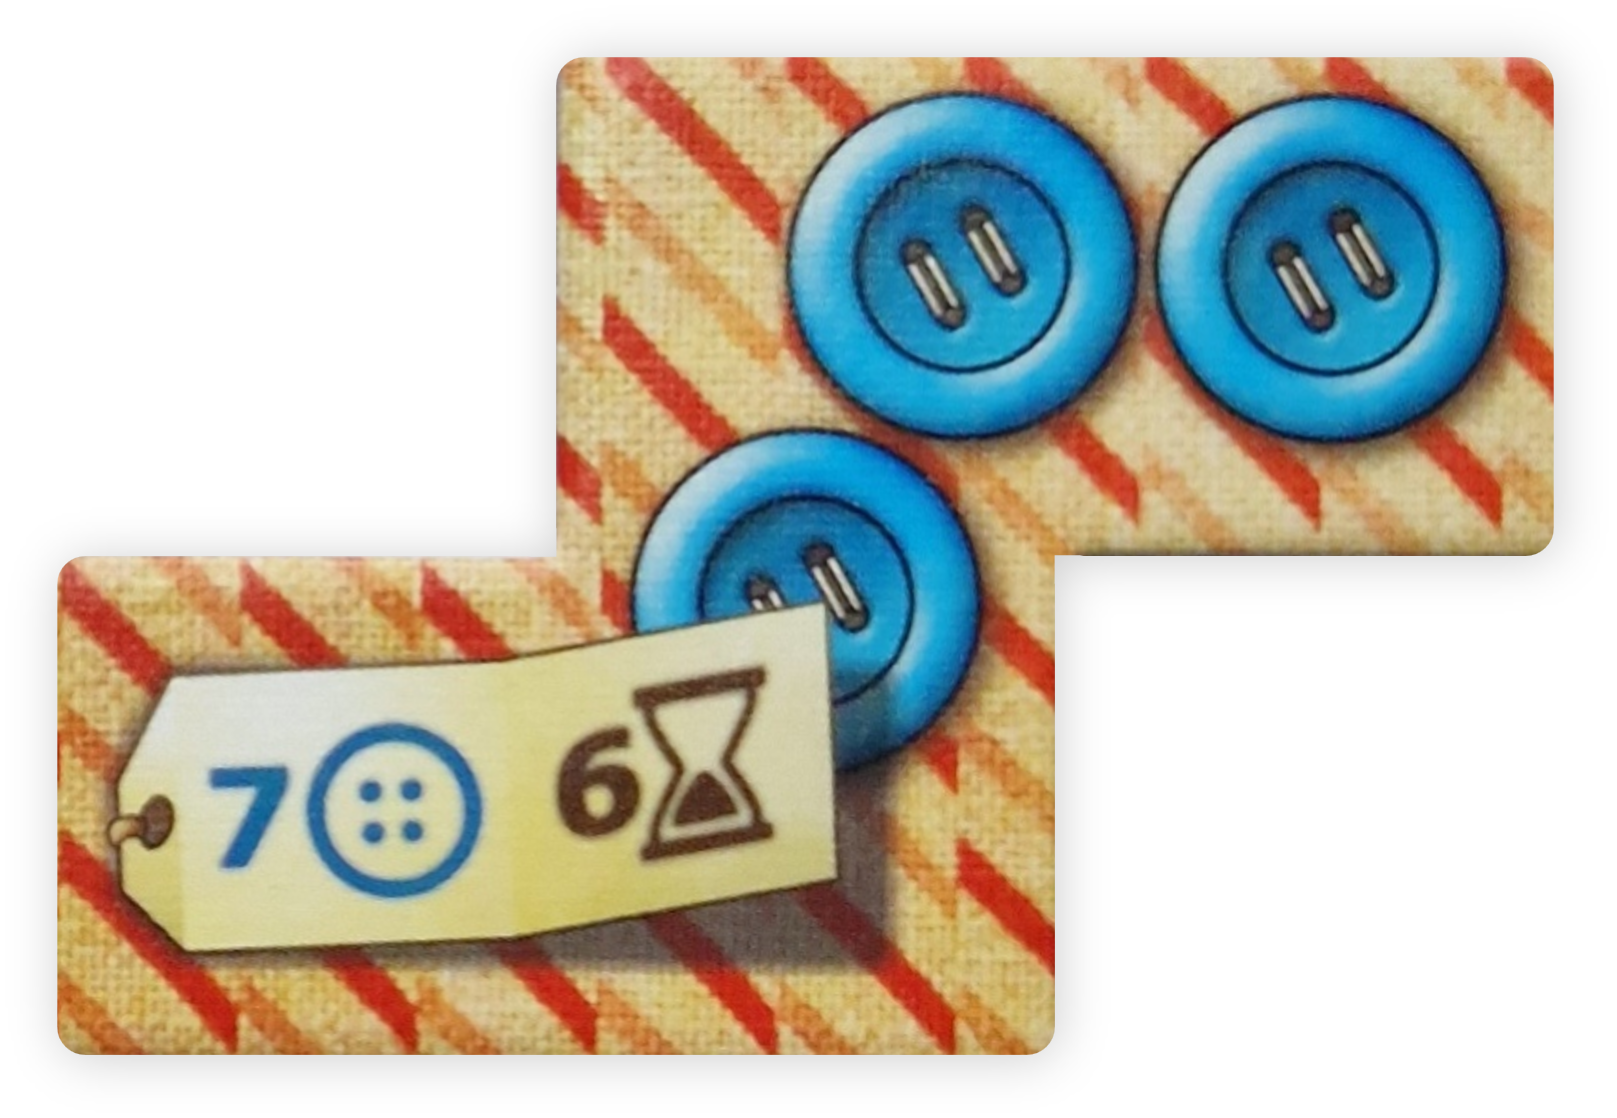
\includegraphics[width=0.2\textwidth]{res/pictures/assets/04-front.png}
    \vspace{-10pt}
    % Das folgende ist ein Trick, um "Abbilgung x.y" in eine
    % eigene Zeile zu packen. Der Text zwischen [ und ] steht
    % im Abbildungsverzeichnis. Der Text darunter wird
    % tatsächlich angezeigt.
    \caption[Flicken mit $V_1\left(F\right) = -2$]{\unskip}
    Flicken mit $V_1\left(F\right) = -2$
    \label{fig:negative-value-patch}
    \vspace*{-0.375cm}
\end{wrapfigure}

Nach Einsetzen aller Flicken in die Value-Funktion ergeben sich für alle Flicken und alle $\alpha > 1$ im Vergleich zu der Laufen-Aktion Werte größer gleicht 1. Somit sind alle \enquote{Flicken nehmen und einfügen} Aktionen vor der vorletzten Knopf-Wertung äquivalent oder öfters der Fall besser als \enquote{Vorrücken und Knöpfe erhalten}. Für $\alpha = 1$ gibt es für den Vergleich $ V_1\left(F\right) - V\left(Walk\right)$ insgesamt 6 Flicken mit dem Ergebnis $\le 0$. Somit kann kurz vor dem Ziel ein Flicken gekauft werden, mit dem Resultat, dass das Endergebnis schlechter ausfällt als nur zu laufen. Da die Summe der Zeitkosten von je 2 dieser 6 Flicken größer als 6 ist, kann jedoch nur genau einer dieser Flicken gekauft werden. Dabei muss darauf geachtet werden, dass auf dem Zeitplan auch genauso viele Felder gelaufen werden, wie der Flicken vorgibt und keine Zeitkosten mit in das Ziel genommen werden. Der in Abbildung \ref{fig:negative-value-patch} dargestellte Flicken besitzt als einziger der Sechs eine Value-Funktion von $-2$ bei $\alpha = 1$ und minimiert somit die Endwertung.

Für Spezialflicken ist die Value-Funktion Konstant $V\left(\text{Spezialflicken}\right) = 2$, da immer genau ein Feld auf dem Ablageplan befüllt wird. Da sich die Wertung somit durch einen Spezialflicken erhöhen würde, sollten für die minimale Wertung keine Spezialflicken eingesammelt werden.

Um nun die minimale Wertung am Ende zu erhalten kann ein Spieler also 47-mal hintereinander laufen und zuletzt den in \ref{fig:negative-value-patch} dargestellten Flicken kaufen. Dadurch ergibt sich für die minimale Wertung am Ende des Spiels eine Wertung von $5 - 2 \cdot 81 + 47 - 7 + 2 \cdot 4 + 3 = -106$ Punkten. Im Gegensatz dazu bringt ein Spielverlauf, bei dem ein Spieler nur läuft eine Endwertung ovn $-104$ Punkten.

\subsection*{Maximale Wertung als Optimierungsproblem}

Mit der Schätzung für die maximale Wertung eines Spielers im vorherigen Abschnitt gibt es einige Probleme.

lässt sich als \acf{ILP} Optimierungsproblem formulieren

\pagebreak

\textbf{Konstanten}

\renewcommand{\arraystretch}{0.6666}

\begin{addmargin}[1em]{0em}
    Knopfkosten der Flicken (\emph{cost}) \vspace*{-10pt}
    \begin{fleqn}
        \begin{align*}
            \begingroup
            \setlength\arraycolsep{1.5pt}
            c = \begin{bmatrix}
                2 & 10 & 5 & 8 & 7 & 4 & 2 & 2 & 2 & 6 & 2 & 1 & 7 & 10 & 4 & 7 & 1 & 5 & 10 & 4 & 1 & 1 & 1 & 3 & 2 & 2 & 3 & 7 & 3 & 5 & 3 & 3 & 0
            \end{bmatrix}^\mathsf{T}
            \endgroup \in \mathbb{N}_0^{33} &
        \end{align*}
    \end{fleqn}
    Zeitkosten der Flicken (\emph{time}) \vspace*{-10pt}
    \begin{fleqn}
        \begin{align*}
            \begingroup
            \setlength\arraycolsep{1.5pt}
            t = \begin{bmatrix}
                1 & 4 & 3 & 6 & 6 & 2 & 1 & 3 & 2 & 5 & 3 & 2 & 2 & 5 & 6 & 4 & 5 & 4 & 3 & 2 & 4 & 3 & 2 & 1 & 2 & 2 & 2 & 1 & 3 & 5 & 6 & 4 & 3
            \end{bmatrix}^\mathsf{T}
            \endgroup \in \mathbb{N}^{33}
        \end{align*}
    \end{fleqn}
    Knopfeinkommen der Flicken (\emph{profit}) \vspace*{-10pt}
    \begin{fleqn}
        \begin{align*}
            \begingroup
            \setlength\arraycolsep{1.5pt}
            p = \begin{bmatrix}
                0 & 3 & 1 & 3 & 3 & 0 & 0 & 0 & 0 & 2 & 1 & 0 & 2 & 3 & 2 & 2 & 1 & 2 & 2 & 1 & 1 & 0 & 0 & 0 & 0 & 0 & 1 & 1 & 1 & 2 & 2 & 1 & 1
            \end{bmatrix}^\mathsf{T}
            \endgroup \in \mathbb{N}_0^{33}
        \end{align*}
    \end{fleqn}
    Fläche der Flicken (\emph{area}) \vspace*{-10pt}
    \begin{fleqn}
        \begin{align*}
            \begingroup
            \setlength\arraycolsep{1.5pt}
            a = \begin{bmatrix}
                2 & 5 & 8 & 6 & 4 & 6 & 6 & 7 & 5 & 4 & 5 & 6 & 6 & 6 & 4 & 6 & 6 & 5 & 5 & 4 & 7 & 3 & 5 & 3 & 4 & 3 & 4 & 5 & 4 & 5 & 6 & 5 & 6
            \end{bmatrix}^\mathsf{T}
            \endgroup \in \mathbb{N}^{33}
        \end{align*}
    \end{fleqn}
    Felder vor den Knopf-Wertungen \vspace*{-10pt} % 0 - 53
    \begin{fleqn}
        \begin{align*}
            \begingroup
            \setlength\arraycolsep{1.5pt}
            b = \begin{bmatrix}
                4 & 10 & 16 & 22 & 28 & 34 & 40 & 46 & 52
            \end{bmatrix}^\mathsf{T}
            \endgroup \in \mathbb{N}^{9}
        \end{align*}
    \end{fleqn}
\end{addmargin}

\textbf{Variablen}

\begin{align*}
    X &= \begin{bmatrix}
        x_{1,1} & \dots & x_{1,9}\\
        \vdots & \ddots & \vdots \\
        x_{33,1} & \dots & x_{33,9}
    \end{bmatrix} & X &\in \{0,1\}^{33 \times 9} \\
    Y &= \begin{bmatrix}
        y_{1,1} & \dots & y_{1,9}\\
        \vdots & \ddots & \vdots \\
        y_{33,1} & \dots & y_{33,9}
    \end{bmatrix} & Y &\in \{0,1\}^{33 \times 9} \\
    z &= \begin{bmatrix}
        z_1 & \dots & z_{33}
    \end{bmatrix}^\mathsf{T} & z &\in \{0,1\}^{33} \\
    \psi &= \begin{bmatrix}
        \psi_1 & \dots & \psi_9
    \end{bmatrix}^\mathsf{T} & \psi &\in \mathbb{N}_0^{9} \text{ insbesondere } \psi_i \ge 0 \\
    \xi &= \begin{bmatrix}
        \xi_1 & \dots & \xi_8
    \end{bmatrix}^\mathsf{T} & \xi &\in \mathbb{N}_0^{8} \text{ insbesondere } \xi_i \ge 0 \\\\
    \lambda && \lambda & \in \{0,1\} \\
\end{align*}



\textbf{Zielfunktion}

\begin{align*}
    \smash{\displaystyle{\maximize_{X,Y,\lambda,\psi}}}\qquad & 5 \tag{\text{Startknöpfe}} \\
    & + 7 \tag{\text{Sonderplättchen}}\\
    & - 2 \cdot 81 \tag{\text{Ablageplanabzug}} \\
    & + p^\mathsf{T}X\vec{1} \tag{\text{Knopfeinkommen maximieren}} \\
    & + 2 \cdot \left(\lambda\cdot 81 + (1 - \lambda) \cdot a^\mathsf{T}X\vec{e_9}\right) \tag{\text{Fläche maximieren}} \\
    & - c^\mathsf{T}X\vec{e_9} \tag{\text{Kosten minimieren}} \\
    & + \psi^\mathsf{T}\vec{1} \tag{\text{Laufen einberechnen}} \\
    \intertext{\hspace{7cm} wobei $\vec{1}$ der Vektor bestehend aus Einsen ist \newline \hspace*{7.3cm} und $\vec{e_i}$ ein kanonischer Einheitsvektor ist.}
\end{align*}

\textbf{Nebenbedingungen}

\begin{addmargin}[1em]{0em}
    Fläche muss kleiner gleich $81$ sein. Keine weitere Optimierung ab $76$ gefüllten Feldern nötig, da Spezialflicken gelegt werden können.
\end{addmargin}
\begin{align*}
   a^\mathsf{T}X\vec{e_9} &\le 81 &\\
   a^\mathsf{T}X\vec{e_9} - 76 + 1 &\le 1000 \cdot \lambda \qquad \text{ bzw. } & a^\mathsf{T}X\vec{e_9} - 76 < 1000 \cdot \lambda \hspace*{1.25cm} \\
   76 \lambda &\le a^\mathsf{T}X\vec{e_9}\\
\intertext{\begin{addmargin}[1em]{0em}
Zeitkosten müssen kleiner gleich $52$ sein, wobei ab $52$ noch genau ein weiterer Flicken gekauft werden kann.
\end{addmargin}}
    t^\mathsf{T}(X\vec{e_9} - z) + \psi^\mathsf{T}\vec{1} &\le 52 &\\
    z^\mathsf{T}\vec{1} &\le 1 &\\
    z_i &\le X_{i,9} - X_{i,8} & i=1,\dots,33\\
\intertext{\begin{addmargin}[1em]{0em}
Bis zu jeder Knopf-Wertung nur so viele Flicken kaufen, wie durch die Zeitkosten erlaubt ist.
\end{addmargin}}
    \left(X\vec{e_1}\ \phantom{ - X\vec{e}_{j-1} } - Y\vec{e_1} \right)^\mathsf{T}t + \psi_1 &\le b_1 \\
    \ \xi_{j-1} + \left(X\vec{e_j} - X\vec{e}_{j-1} - Y\vec{e_j} \right)^\mathsf{T}t + \psi_j &\le b_j & j=2,\dots,9\\
    b_j &\le \xi_j &j=1,\dots,8\\
    t^\mathsf{T}X\vec{e_1} + \psi_1 &\le \xi_1 \\
    \xi_{j-1} + t^\mathsf{T}\left(X\vec{e_j} - X\vec{e}_{j-1}\right) + \psi_j &\le \xi_j &j=2,\dots,8\\
    \left(Y\vec{e_j}\right)^\mathsf{T}\vec{1} &\le 1 & j=1,\dots,9 \\
    Y_{i,j} &\le X_{i,j} & i=1,\dots,33\quad j=1\phantom{,\dots,9} \\
    Y_{i,j} &\le X_{i,j} - X_{i,j-1} & i=1,\dots,33\quad j=2,\dots,9 \\
\intertext{\begin{addmargin}[1em]{0em}
Knopfvorrat muss größer gleich $0$ vor allen Knopf-Wertungen sein sein.
\end{addmargin}}
    5 + \sum_{k=1}^{j-1}\left( p^\mathsf{T}X\vec{e_k} + \psi_k \right) &\ge c^\mathsf{T}X\vec{e_j} & j=1,\dots,9\\
\intertext{\begin{addmargin}[1em]{0em}
Und eine weitere Bedingungen, um abzusichern, dass Flicken die früher genommen wurden auch später noch existieren. Weiterhin die korrekte bereichnung von $\psi$ dem Laufen.
\end{addmargin}}
    X_{i,j} &\le X_{i,j+1} & i=1,\dots,33\quad j=1,\dots,8 \\
    \psi_j &\ge b_j - t^\mathsf{T}X\vec{e_j} &j=1,\dots,9 \\
\intertext{\begin{addmargin}[1em]{0em}
    Omega.
    \end{addmargin}}
    \omega_i &\le X_{i,9} & i=1,\dots,33 \\
    \omega^\mathsf{T}\vec{1} &\le 33 \cdot \lambda \\
    X_{i,9} + \lambda - 1 &\le \omega_i & i=1,\dots,33 \\
\end{align*}



\begin{align*}
    \smash{\displaystyle{\maximize_{X,Y,\lambda,\psi}}}\qquad & 5 +7 - 2 \cdot 81 + p^\mathsf{T}X\vec{1}  \\
    & + 2 \cdot 81 \cdot \lambda \\
    & + 2 \cdot a^\mathsf{T}X\vec{e_9} \\
    & + 2 a^\mathsf{T}\omega \\
    & - c^\mathsf{T}X\vec{e_9} + \psi^\mathsf{T}\vec{1}  \\
\end{align*}

\renewcommand{\arraystretch}{1}

\pagebreak


\subsection*{Betrachtung der Spiel-Komplexität}

TODO:

% sum k=1 to n of P(n, k) = n! / (n-k)! = 36! / (36-k)! = 36! / (36-36)! = 36! / 0! = 36!


% import math
% result = 0
% for k in range(1, n+1):
%     result += math.factorial(36) // math.factorial(36 - k)
% print(result)

% P(3) = 15
% P(2) = 6
% P(1) = 3

% 1*6+3*2+3*1=15

% (1,2,3) * 3!
% (1,2) * 2!
% (1,3) * 2!
% (2,3) * 2!
% (1) * 1!
% (2) * 1!
% (3) * 1!
% ()  * 0!

% TODO: hyperreferencen für Komplexitätsparameter (e.g. Spielbaumkomplexität) in Formelsammlung einfügen

Der komplexitätstheoretische Rechenaufwand für Patchwork ist, wie auch für TicTacToe oder Schach, $\mathcal{O}(1)$, da das Spiel eine feste Brettgröße besitzt und somit nur endlich viele Zustände zulässt. Somit ist es theoretisch möglich eine Tabelle zu konstruieren, bei der zu jedem Zustand angegeben wird, was die beste Aktion ist. Praktisch ist dies aber im Gegensatz zu TicTacToe durch die große Menge an Zuständen nicht umsetzbar.

Eine Schätzung für die Spielbaumkomplexität wird im nachfolgenden Abschnitt vorgenommen.

\section{Auswertung empirischer Daten}

Um die vorangegangenen Komplexitätsbetrachtungen genauer einordnen zu können und um gleichzeitig eine realistischere Betrachtung von Patchwork zu erhalten, werden 10 Millionen Spiele von Patchwork aufgenommen und ausgewertet. Dabei treten 2 Computer gegeneinander an, welche für ihren Zug immer eine zufällige Aktion aus allen möglichen Aktionen auswählen (siehe Kapitel \ref{section:erstellung-ansatz-a}). So sollten die 10 Millionen Spiele eine möglichst unverzerrte Datenverteilung enthalten, bei der keine bestimmte Spielkonfiguration bevorzugt wird.

% MEAN: 42.8176
% MEDIAN: 43.0
% MIN: 34 (Count: 4000)
% MAX: 54 (Count: 2000)
% VAR: 8.031931043193113
% STDEV: 2.834066167751401
\begin{figure}[!ht]
    \centering
    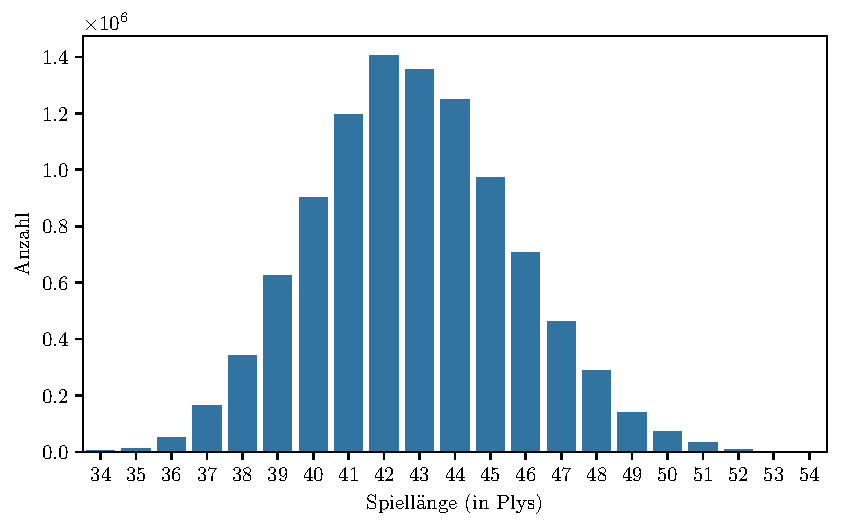
\includegraphics[width=0.7\textwidth]{res/pictures/plots/game_lengths.pdf}
    % \vspace*{-0.5cm}
    \caption{Spiellänge der 10 Millionen Spiele in \hyperref[text:ply]{\emph{Plys}}}
    \label{fig:plot-game-length-10-million}
\end{figure}

Die durchschnittliche Spiellänge, gemessen in \hyperref[text:ply]{\emph{Plys}}, beträgt ${\approx}42{,}8176$. Die kürzesten Spiele der Messung sind nach 34 \hyperref[text:ply]{\emph{Plys}} beendet. Das bedeutet nicht, dass es keine Spiele geben kann, welche kürzer gehen, sondern dass diese in der Messung nicht vorhanden sind. Zu sehen ist das an der maximalen Länge. Hier wurden nur Spiele bis zu einer Länge von 54 \hyperref[text:ply]{\emph{Plys}} erreicht, während wie in »\nameref{subsection:analyse-laenge-des-spiels}« gezeigt auch ein Spielverlauf mit bis zu 63 \hyperref[text:ply]{\emph{Plys}} möglich ist. Die gesamte Verteilung der Spiellänge der empirischen Messung ist in Diagramm \ref{fig:plot-game-length-10-million} zu sehen.

% MEAN: 83.65933586478253
% MEDIAN: 11.0
% MIN: 1 (Count: 130760000)
% MAX: 1345 (Count: 2000)
% VAR: 22351.213723901034
% STDEV: 149.50322312211543
\begin{wrapfigure}{r}{0.55\textwidth}
    \vspace*{-0.75cm}
    \centering
    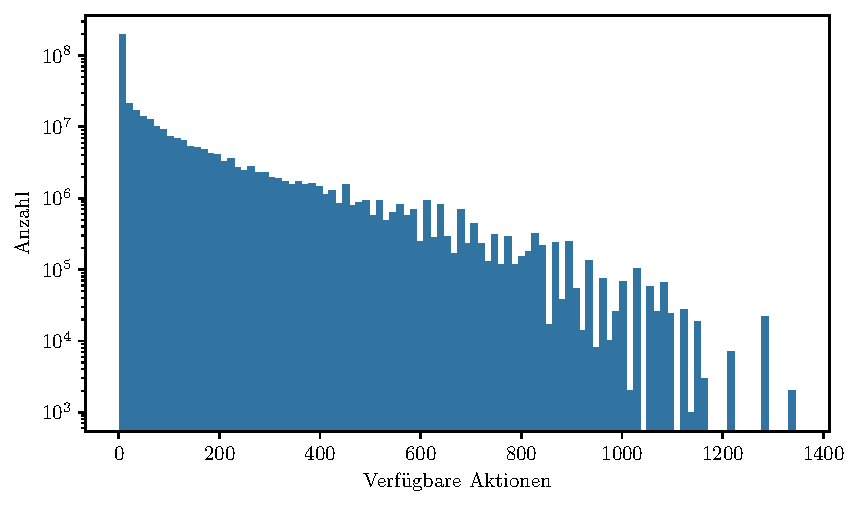
\includegraphics[width=0.549\textwidth]{res/pictures/plots/available_actions.pdf}
    % \vspace{-10pt}
    \caption[Verteilung der verfügbare Aktionen]{\unskip}
    Verteilung der verfügbare Aktionen
    \label{fig:plot-available-actions-10-million}
    \vspace*{-0.85cm}
\end{wrapfigure}

Im Gegensatz zu der normalverteilten Spiellänge, ist die Verteilung der verfügbaren Aktionen, wie in Diagramm \ref{fig:plot-available-actions-10-million} dargestellt ist, stark rechtsschief. Im Diagramm sind dabei keine Aktionen für das Platzieren von Spezialflicken aufgenommen und die Aktionen sind in einer logarithmischen Skala dargestellt. Es existieren deutlich mehr Aktionen mit weniger Möglichkeiten und die durchschnittliche Anzahl an verfügbaren Aktionen liegt bei ${\approx}83{,}66$. Diese rechtsschiefe lässt sich auch leicht erklären: Sobald ein Flicken zu viele Knöpfe kostet oder auf dem Ablageplan keinen Platz findet, fallen auf einen Schlag ungefähr $\sfrac{1}{3}$ der Aktionen weg. Weiterhin fallen immer mehr Platzierungsmöglichkeiten weg, je voller der Ablageplan eines Spielers ist.

\subsection*{Schätzung der Spielbaumkomplexität}

Mit den empirischen Daten lässt sich eine grobe Schätzung für die Komplexität des Spielbaums in Patchwork erstellen, wobei der durchschnittliche Verzweigungsfaktor mit der durchschnittlichen Spiellänge potenziert wird \cite[S. 160]{1194.SearchAndAiInGames}.

% \vspace*{-1cm}
\begin{align}
    \label{eqn:gtc-patchwork-branch-estimation}
    \text{\acsp{GTC}}(Patchwork) & \approx b^d \approx {83{,}6593}^{42{,}8176} \approx 2{,}08 \cdot 10^{82} \\[2pt]
    \tag*{$\text{mit }           b = \text{durchschnittlicher Verzweigungsfaktor}$}                         \\
    \tag*{$\phantom{\text{mit }} d = \text{durchschnittliche\phantom{r} \rlap{Spiellänge}\phantom{Verzweigungsfaktor}}$}
\end{align}

Die in \ref{eqn:gtc-patchwork-branch-estimation} resultierende Schätzung von $2{,}08 \cdot 10^{82}$ ist dabei jedoch wahrscheinlich zu groß. Der Median der verfügbaren Aktionen beträgt im Gegensatz zum Durchschnitt nur $11$. Durch einzelne Zustände mit sehr vielen verfügbaren Aktionen wird der Durschnitt angehoben, obwohl in den meisten Zuständen nur eine oder wenige Aktionen möglich sind.

Eine weitere genauere Schätzung für die Komplexität des Spielbaums kann nach A. und D. Yong gefunden werden. Dazu wird ein Spiel mit $N$ \hyperref[text:ply]{\emph{Plys}} gespielt, wobei die einzelnen Aktionen mittels einer Gleichverteilung ausgewählt werden. In jedem \hyperref[text:ply]{\emph{Ply}} $i$ werden dabei die Anzahl der möglichen Aktionen $c_i(g)$ gespeichert. Aus der Multiplikation all dieser Verzweigungen ergibt sich die Zufallsvariable $X(g)$ als Schätzung für die Komplexität des Spielbaums. Um nun eine möglichst akkurate Schätzung zu erhalten, wird dieser Prozess in vielen unabhängigen Durchläufen wiederholt und der Mittelwert wie in Formel \ref{eqn:gtc-patchwork-avg-estimation} gebildet. Mit $n \to \infty$ nähert sich diese Schätzung immer mehr der tatsächlichen Komplexität des Spielbaums an. \cite{2019.GameTreeComplexityEstimation}

\begin{equation}
    \label{eqn:gtc-patchwork-avg-estimation}
    \begin{aligned}
        X(g)                         & = \prod\nolimits_{j=1}^{N} c_j(g)         \\[15pt]
        \text{\acsp{GTC}}(Patchwork) & \approx \frac{1}{n} \sum_{i=1}^{n} X(g_i) \\[1pt]
                                     & \approx 1{,}68 \cdot 10^{38}
    \end{aligned}
\end{equation}

Als unabhängige Stichproben der Zufallsvariable $X$ können die aufgenommenen 10 Millionen Spiele eingesetzt werden. Somit ergibt sich eine Schätzung der Spielbaumkomplexität von $1{,}68 \cdot 10^{38}$.
